\documentclass[aspectratio=1610]{beamer}
% \documentclass{article}
% 
\usepackage[utf8]{inputenc}
\usepackage[spanish,english]{babel}
\usepackage{graphicx}
\usepackage{amsmath}
\usepackage[left=2cm,right=2cm,bottom=2cm,top=2cm]{geometry}
\usepackage{amssymb}
\usepackage{hyperref}
\hypersetup{
    colorlinks=true,
    linkcolor=blue,
    filecolor=magenta,
    urlcolor=blue,
}
\usepackage{mathrsfs}
\usepackage{amsfonts}
\usepackage{amsthm}
\usepackage{physics}
\usepackage{siunitx}
\usepackage{cancel}
\usepackage{caption}
\usepackage{subcaption}
\usepackage{multicol}
\usepackage{color}
\usepackage{pdfpages}
\usepackage{empheq}
\usepackage{feynmf}
\usepackage{tikz}
\usepackage{titlesec}
\usepackage{mathtools}

\decimalpoint

\setlength{\columnseprule}{.5pt}
\def\columnseprulecolor{\color{black}}

\graphicspath{{images/}}

\usepackage{setspace}
\usepackage{gensymb}
\usepackage{mathpazo}
\usepackage{authblk}
\usepackage{fancyhdr}

\usepackage[utf8]{inputenc}
\usepackage{amsmath}
\usepackage{amsfonts}
\usepackage{amssymb}
\usepackage{graphicx,fancybox}
\usepackage{babel}
\usepackage{minted}
\usepackage{wrapfig}
\usepackage{verbatim}
\usepackage{appendixnumberbeamer}
\usepackage{hyperref}
\usepackage{physics}
\hypersetup{
	colorlinks=true,
	linkcolor=blue,
	filecolor=magenta,
	urlcolor=blue,
}


\graphicspath{{images/}}

\setbeamertemplate{footline}[frame number]
\beamertemplatenavigationsymbolsempty
\usetheme{Madrid}

\addtobeamertemplate{footline}{\hypersetup{allcolors=.}}{}
\definecolor{uprmgreen}{RGB}{51, 113, 55}

\usecolortheme[named=uprmgreen]{structure}

% \usefonttheme{professionalfonts}
% \usepackage{mathpazo}
% \renewcommand\familydefault{\rmdefault}

\title[EMJ and ML4TkDQM]{Trigger Studies for the Emerging Jets Analysis \\and Machine Learning for Tracker DQM \\at the CMS Experiment}
% for documents
% \author[1]{Guillermo Fidalgo Rodríguez} %[1] is to indicate connection with affil institute
% \author{Tetiana}
% \author{Roy}
% \affil[1]{University of Puerto Rico - Mayagüez, Physics Department}

%%%
% for beamer
\author[GAFR]{Guillermo A. Fidalgo Rodríguez}
\institute[UPRM]{University of Puerto Rico -- Mayagüez}
% Multiple logos
\titlegraphic{
    
\includegraphics[height=1.5cm]{uprm_logo.png}
    % \hspace{2cm}
    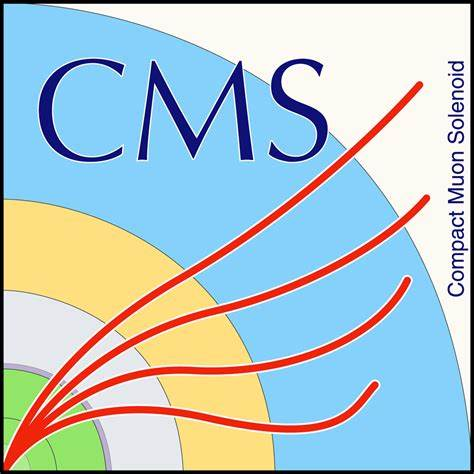
\includegraphics[height=1.46cm]{CMS_logo.jpg}
    % \hspace{2cm}
    
\includegraphics[height=1.5cm]{LPC_logo.png}
    % \hspace{2cm}
    \hfill
    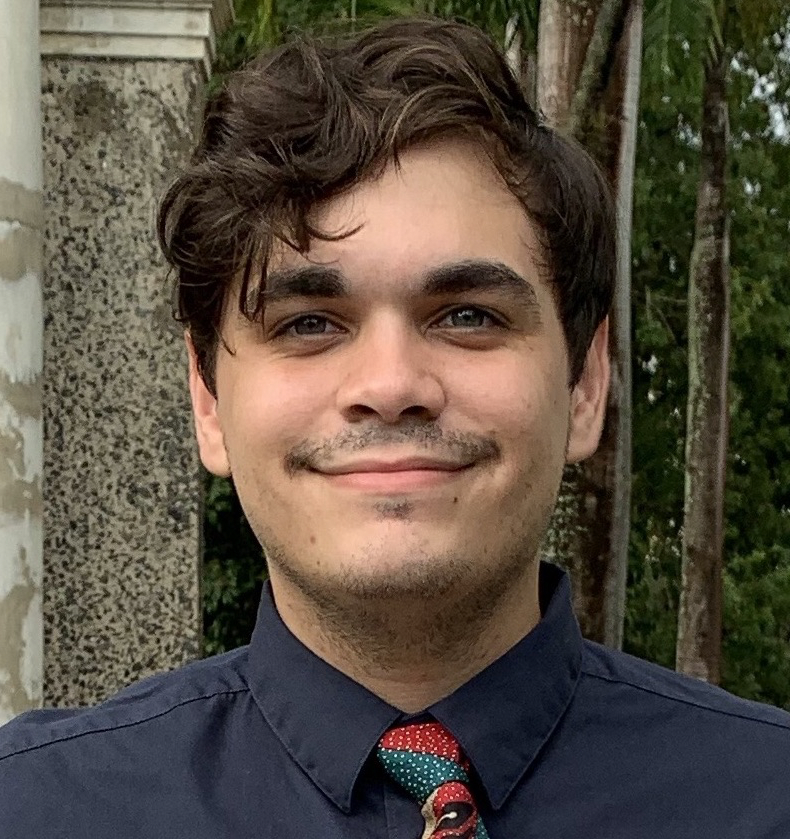
\includegraphics[width=2.7cm]{Guillermo-Grad.png}
}
\date{April 30, 2024}
\begin{document}

\maketitle

\begin{frame}
	% \Huge
	\tableofcontents
\end{frame}

\section{Introduction}

\begin{frame}{Standard Model of Particle Physics}
	\begin{columns}

		\column{.5\textwidth}
		\begin{itemize}
			\item The most successful theory we have
			      \vspace*{1cm}
			\item Predicted the famous Higgs Boson discovered in 2012 (Nobel Prize)
			      \vspace{1cm}
			\item Not complete, we still have more questions
		\end{itemize}
		\column{.5\textwidth}
		\begin{figure}
			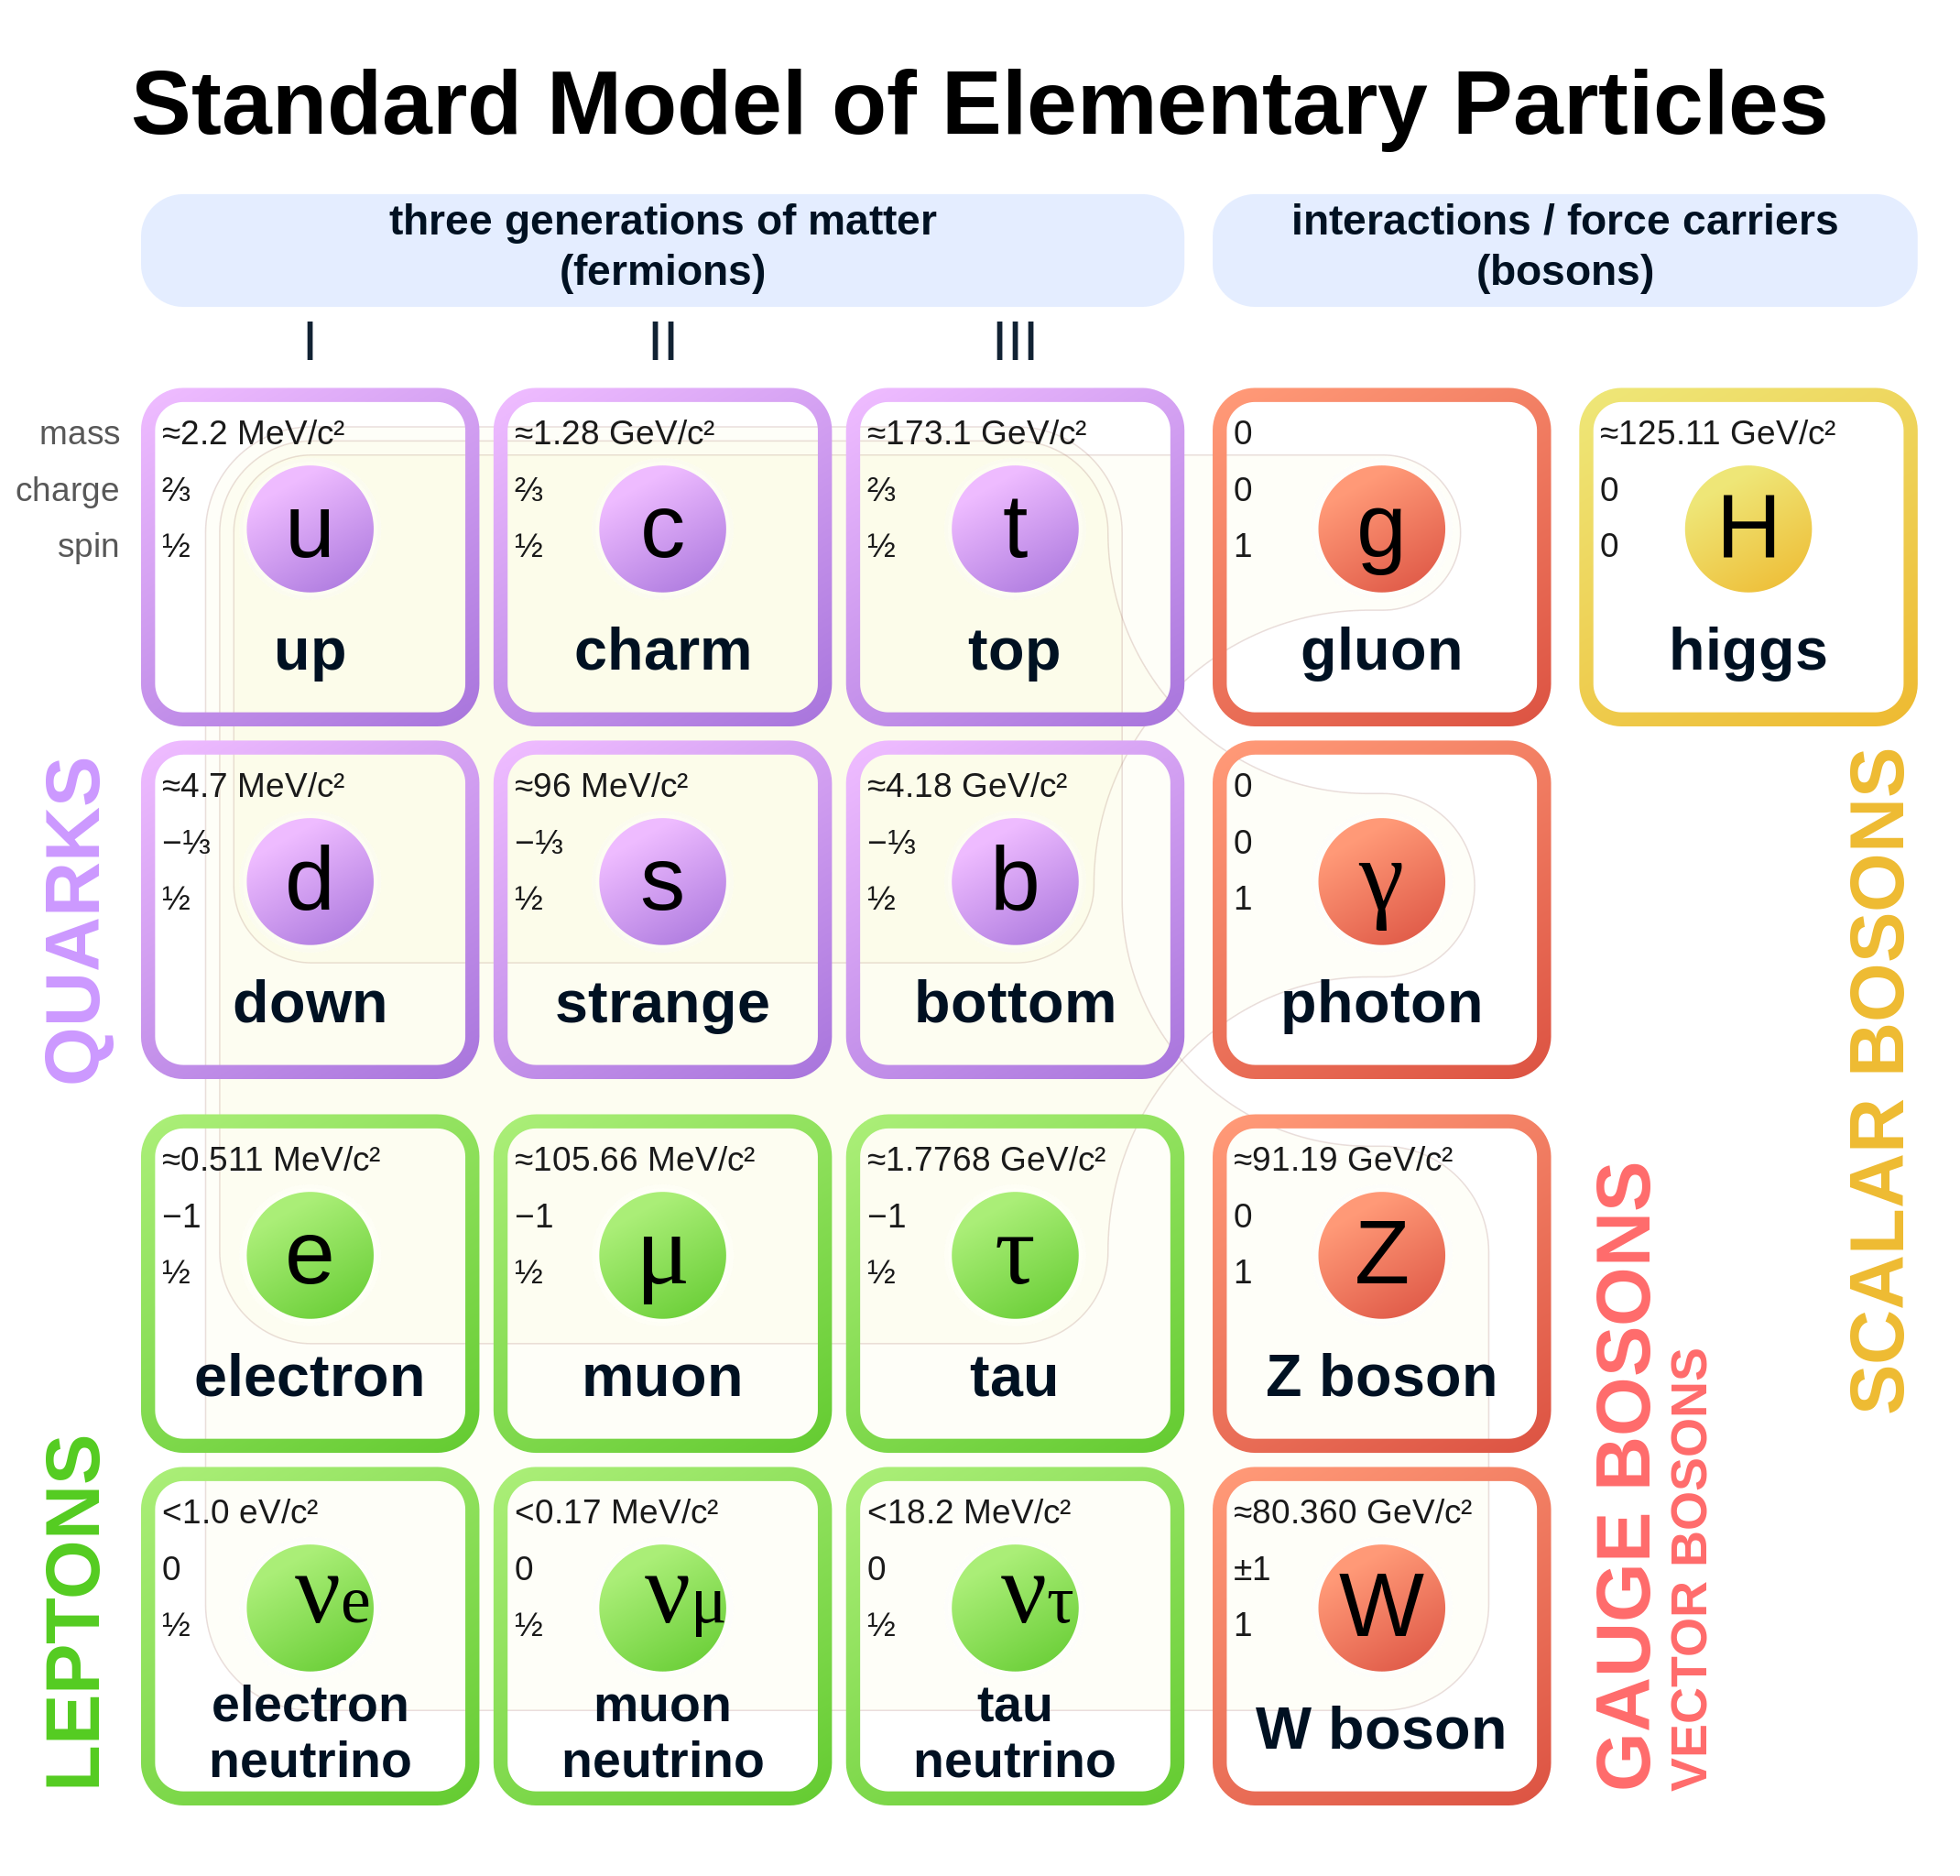
\includegraphics[width=\linewidth]{Standard_Model.png}
		\end{figure}
	\end{columns}
\end{frame}

\begin{frame}{What do we want to accomplish?}
	\begin{itemize}
		\item We want to explain why so much of our Universe is filled with exotic kinds of matter and energy
	\end{itemize}
	\begin{figure}
		\centering
		\begin{subfigure}{0.45\linewidth}
			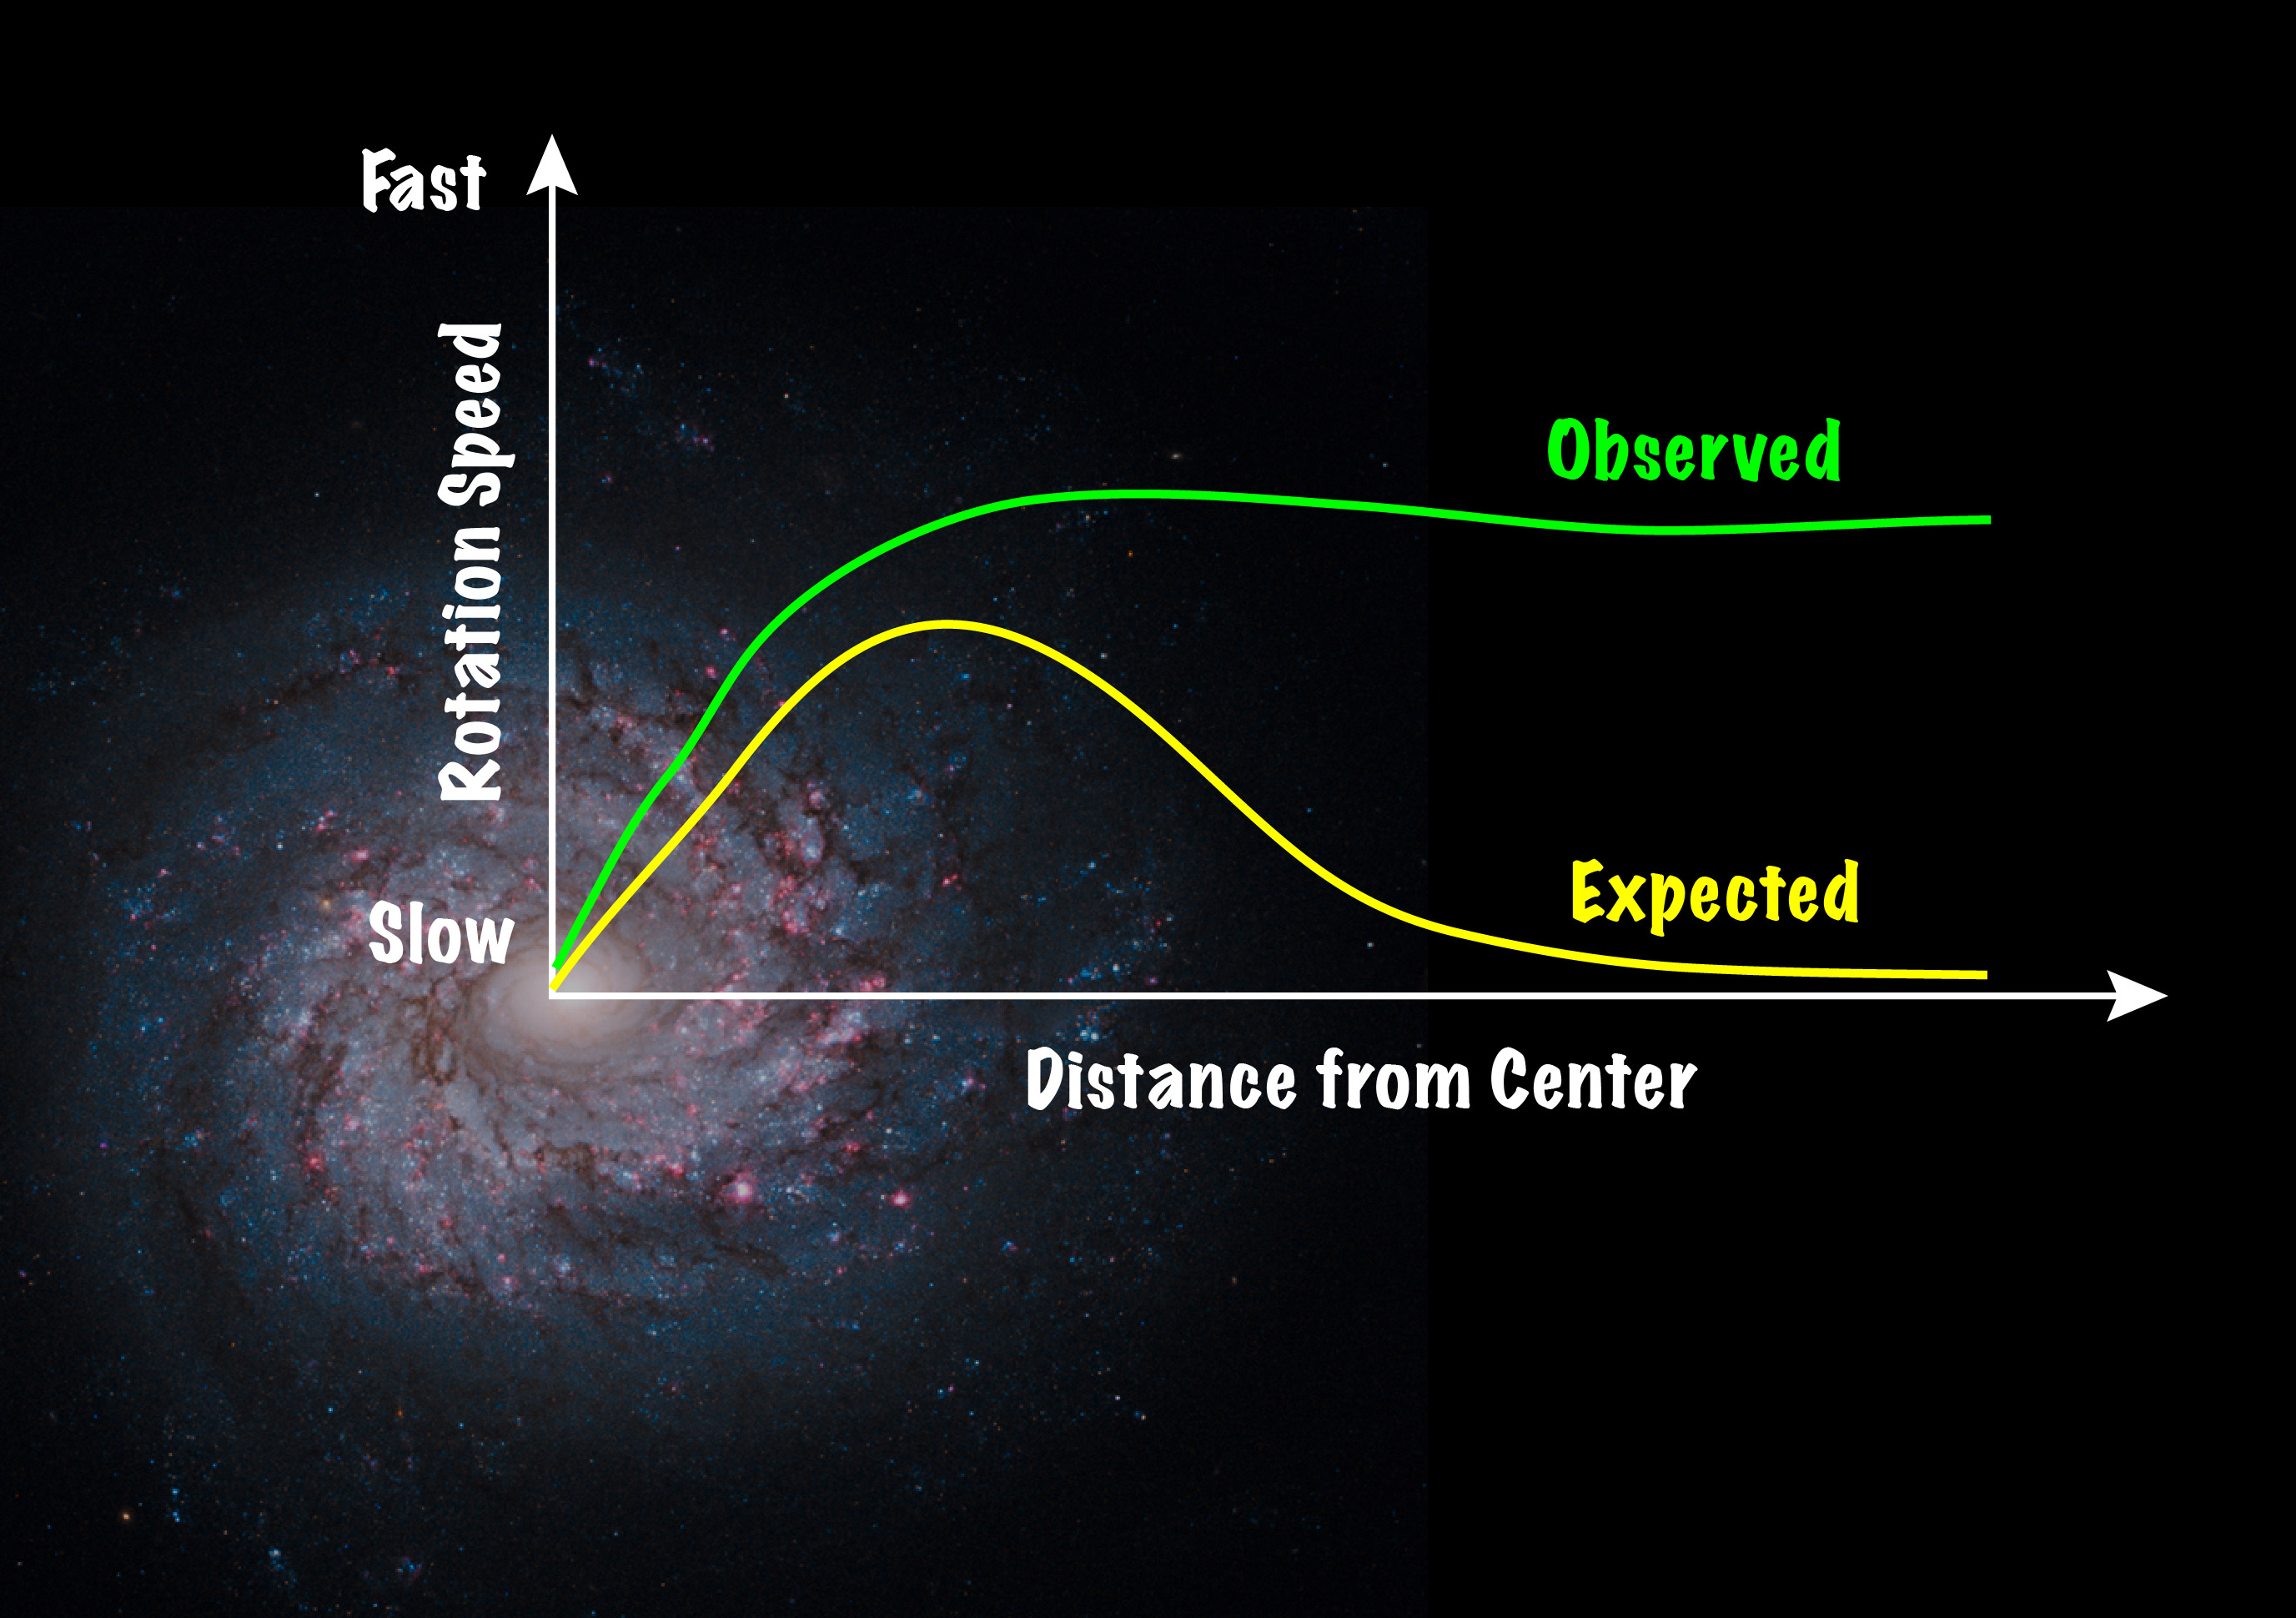
\includegraphics[width=\linewidth]{galaxyrotationcurve.jpg}
			% \caption{Expected vs Observed rotational speed of mass in a galaxy w.r.t. distance from galaxy center.}
		\end{subfigure}
		\begin{subfigure}{0.45\linewidth}
			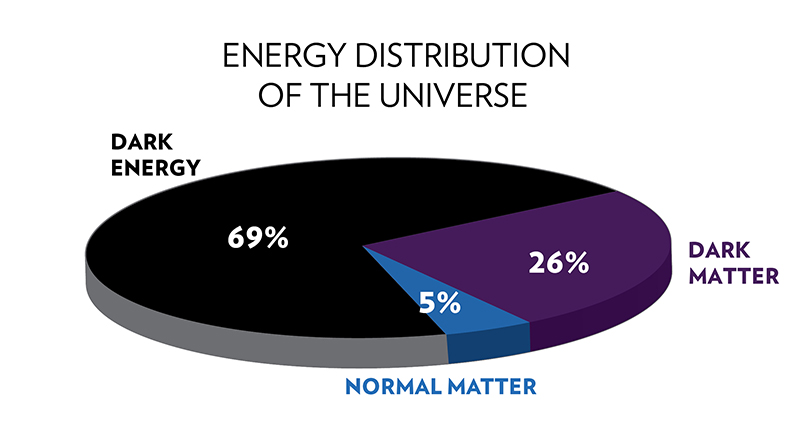
\includegraphics[width=\linewidth]{Energy_dist_pie.jpg}
		\end{subfigure}
	\end{figure}
\end{frame}

\begin{frame}{How do we accomplish it?}
	\begin{columns}
		\column{.45\linewidth}
		\begin{itemize}
			\item In Particle Physics, scientists use the most complex machinery to explore and describe the universe
			\item We accelerate protons to near light-speed to simulate energies of the Big Bang
		\end{itemize}
		\begin{figure}
			\centering
			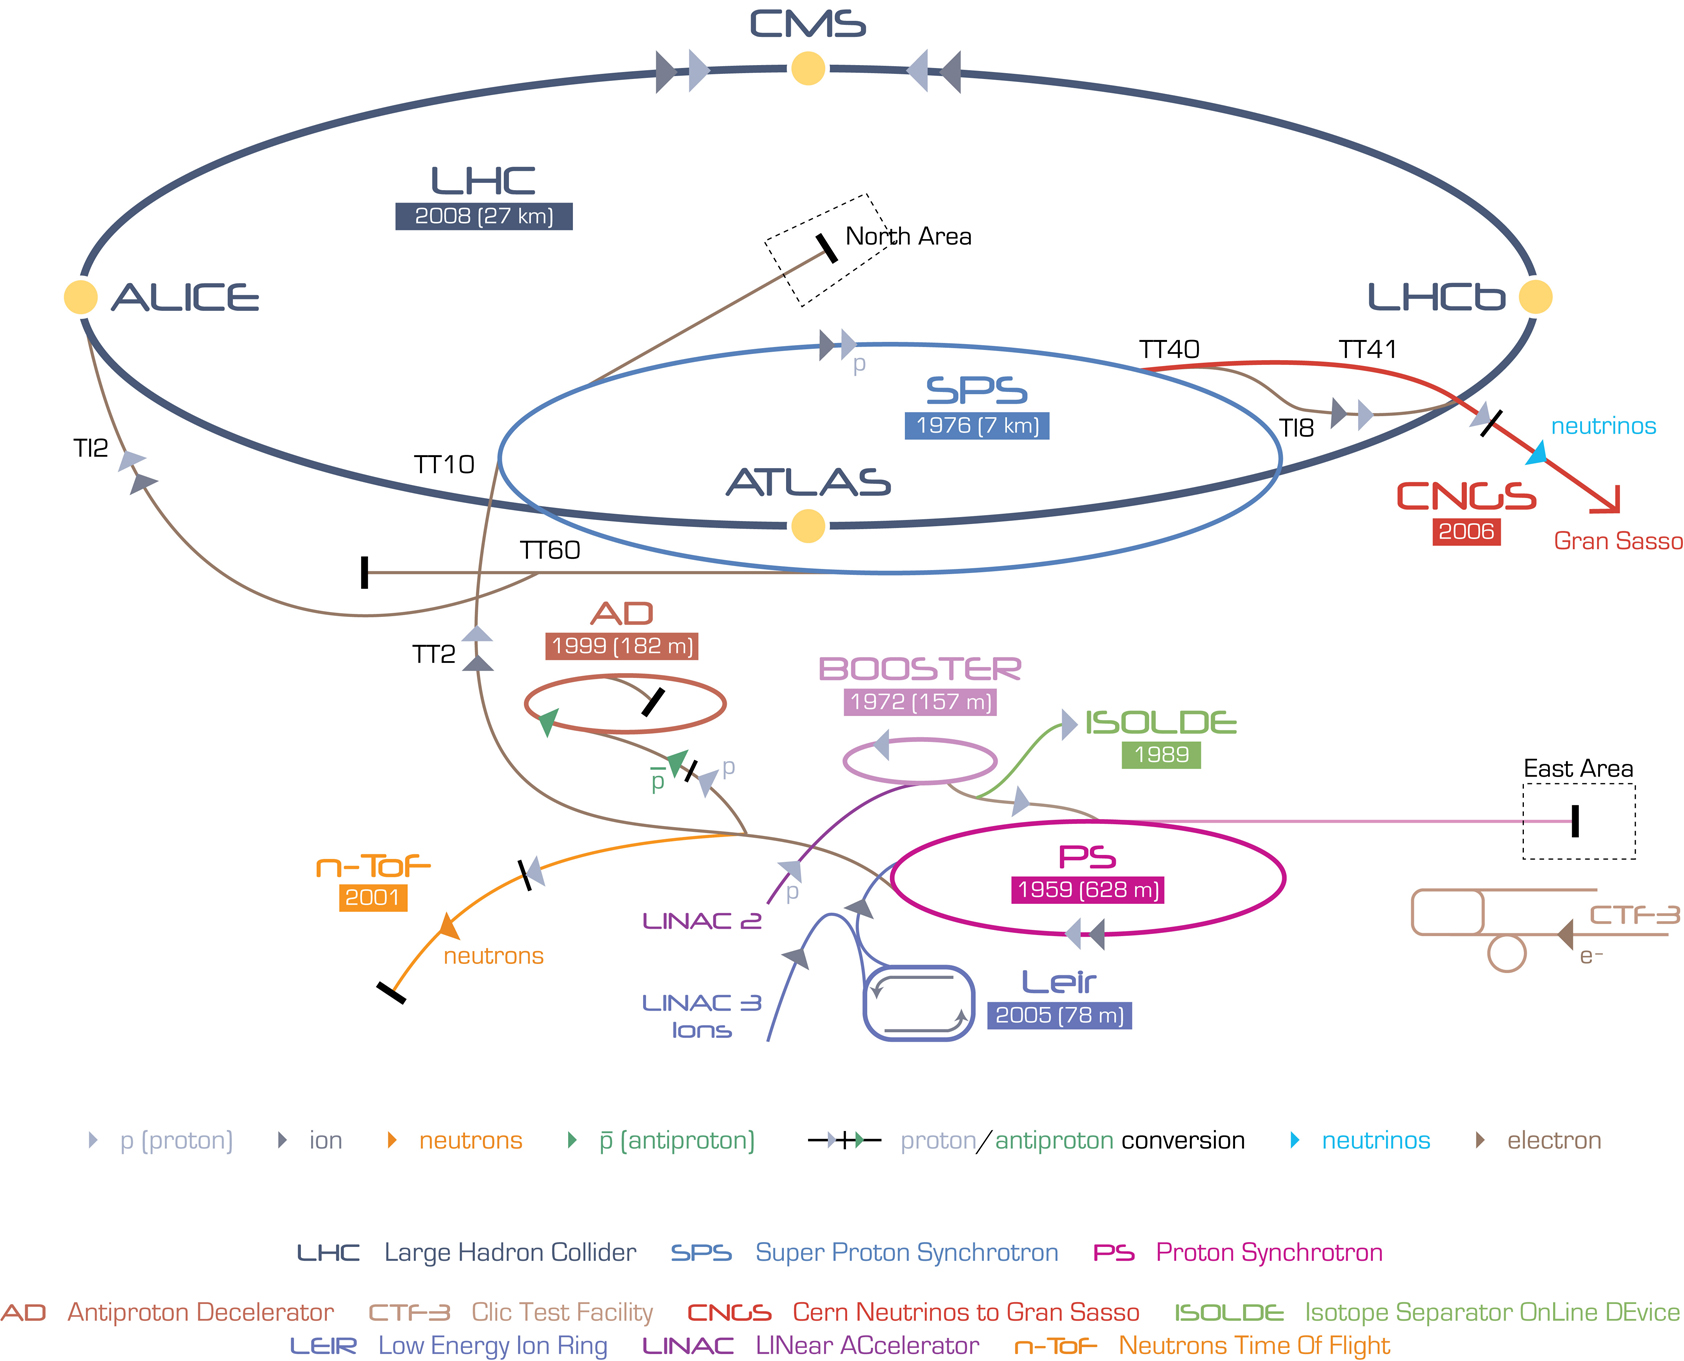
\includegraphics[width=\linewidth]{Cern-Accelerator-Complex.jpg}
		\end{figure}
		\column{.56\linewidth}
		\begin{figure}
			\centering
			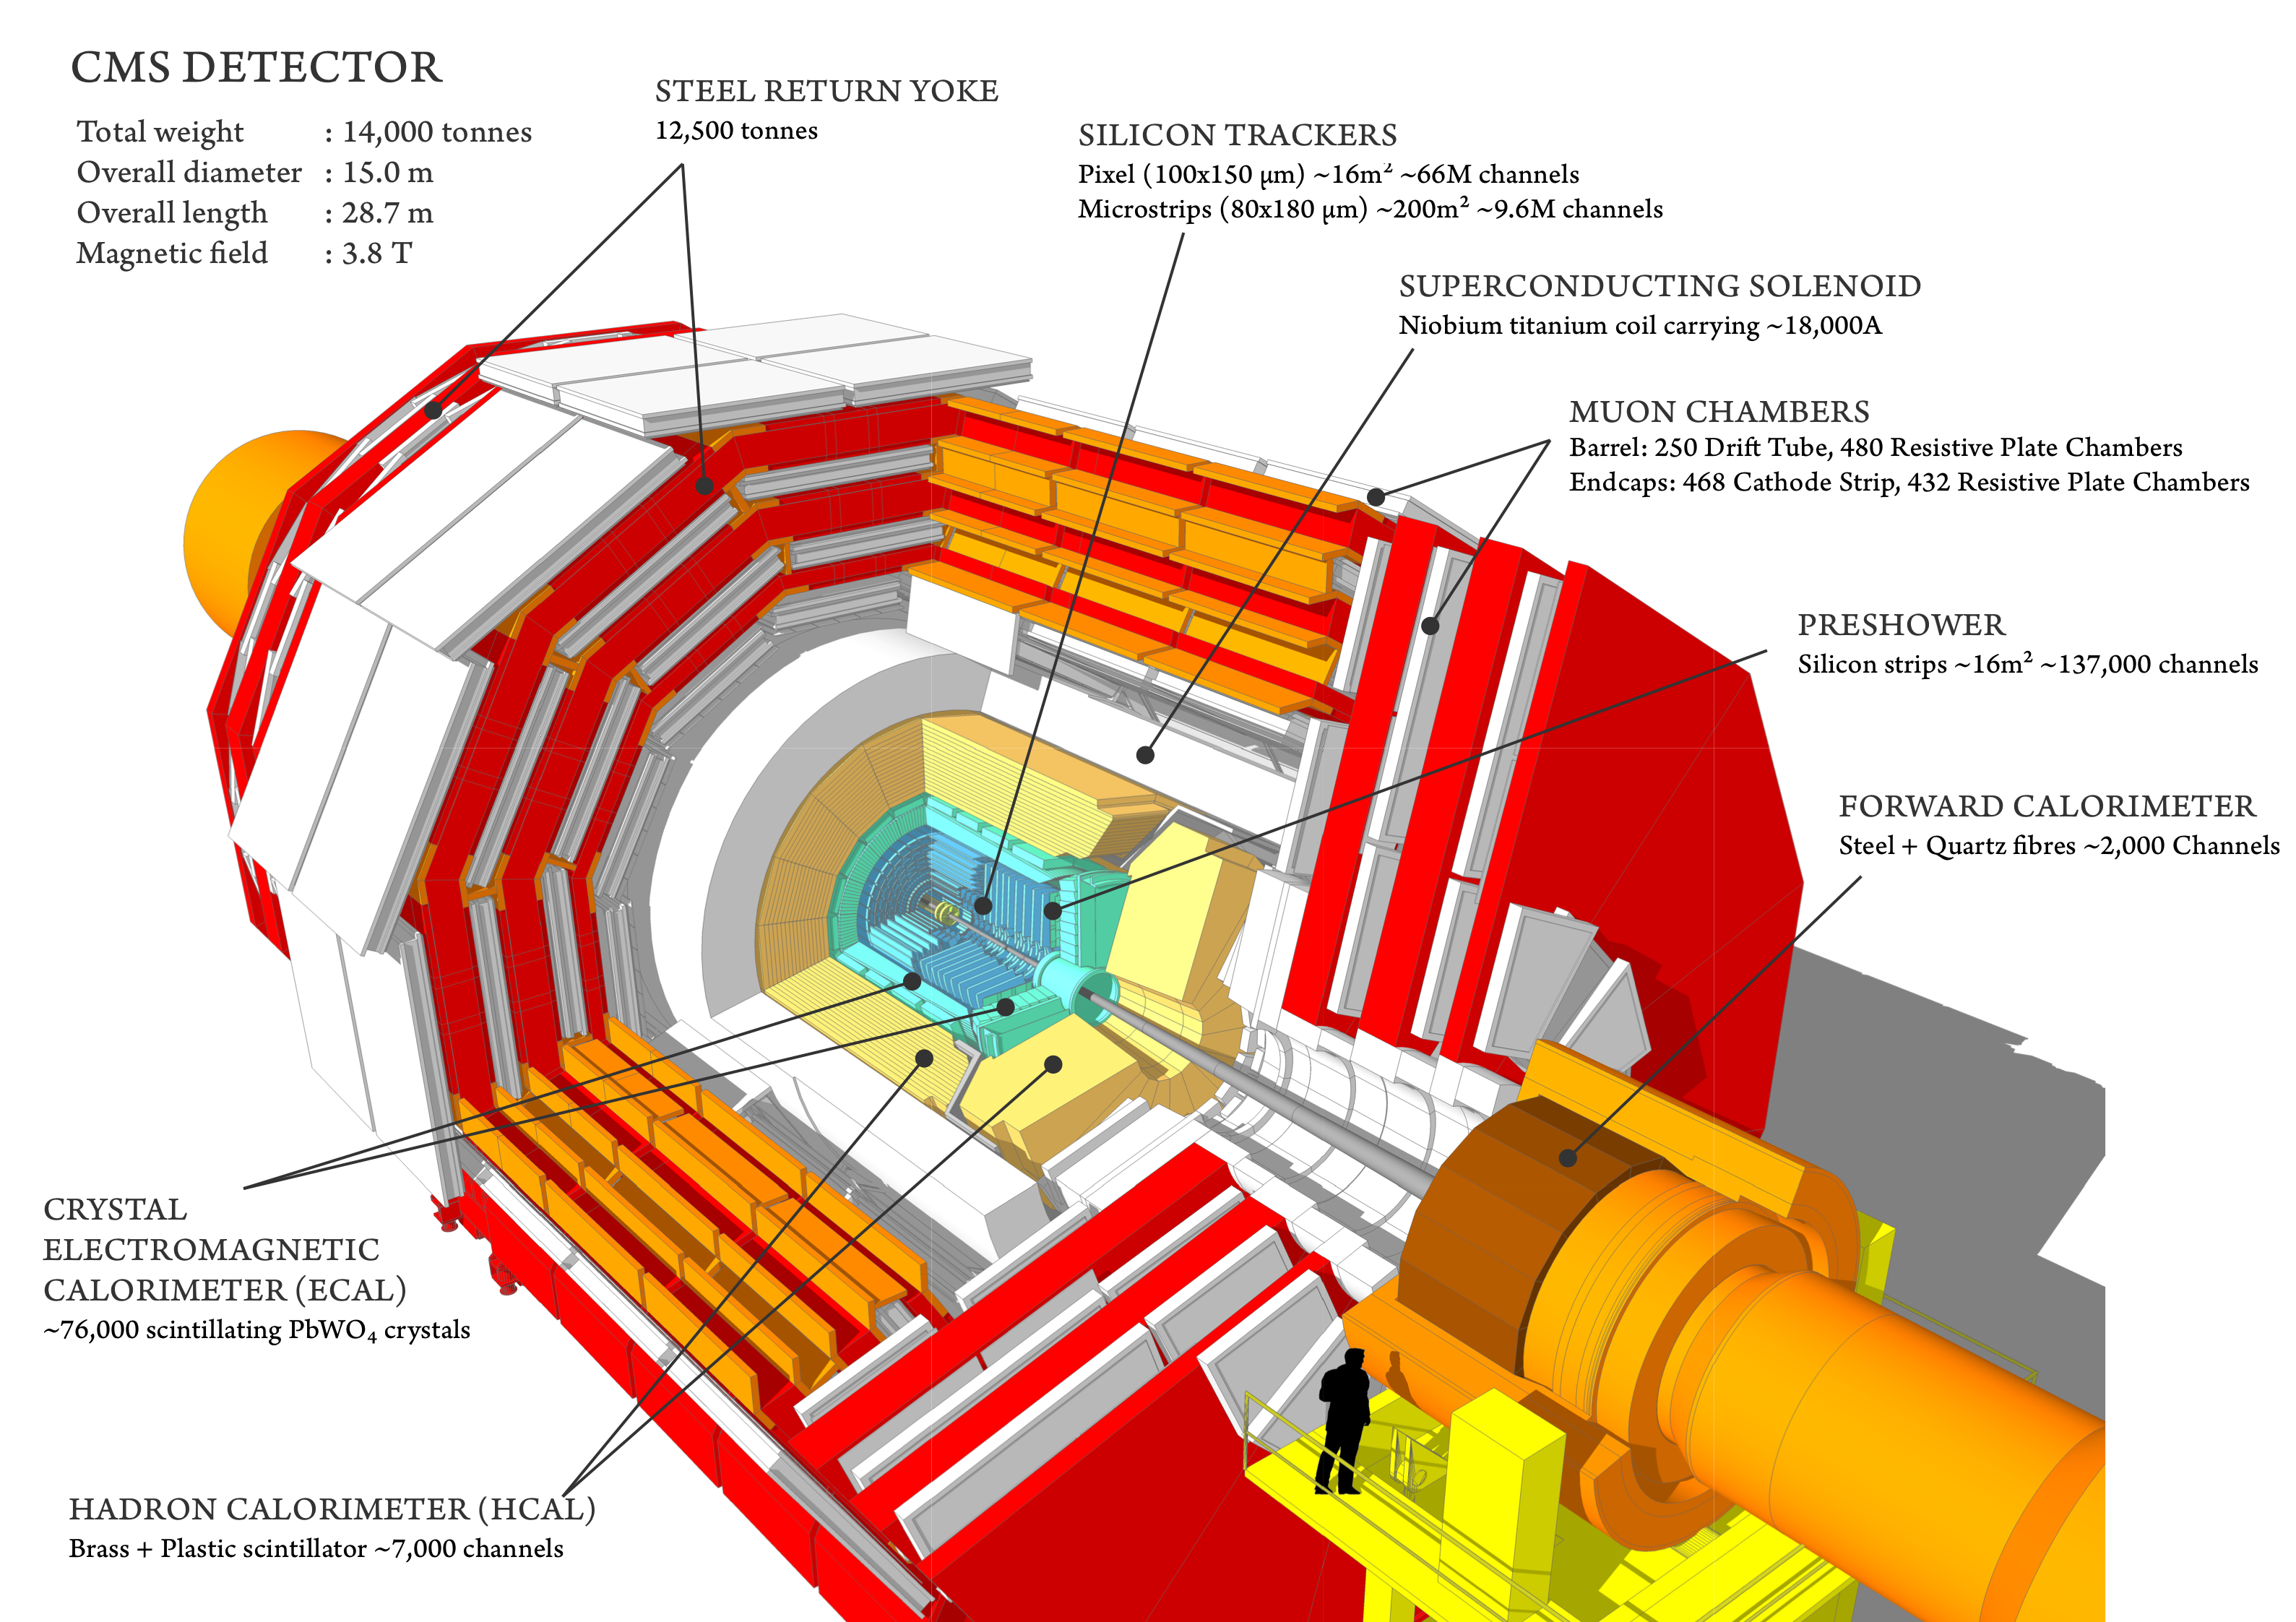
\includegraphics[width=\linewidth]{CMSLayout.png}
		\end{figure}
	\end{columns}
\end{frame}

\begin{frame}{CMS Detector}
	\begin{itemize}
		\item CMS is multipurpose with an onion-like structure
		\item Has 3.8 T magnetic field
		\item Precise tracking system
		\item Able to record events at a rate of 40 MHz but this is filtered with the Trigger system
	\end{itemize}
	\begin{figure}
		\centering
		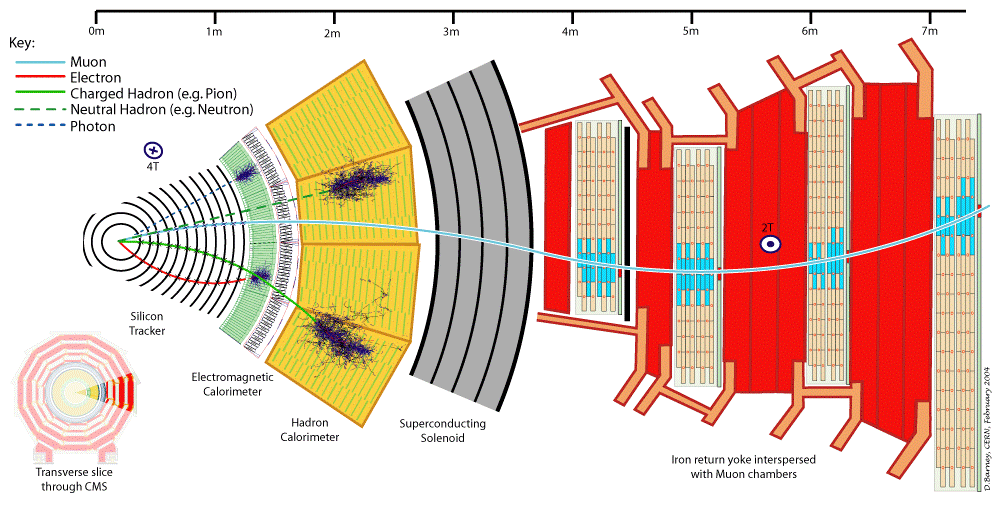
\includegraphics[width=.7\linewidth]{CMSLayers.png}
	\end{figure}
\end{frame}

\begin{frame}
	\frametitle{Trigger System in CMS}
	\begin{itemize}
		\item Responsible for selecting ``intersting'' events
		\item Two tier trigger system -- L1 and HLT
		\item L1 -- Calorimeters and Muon Detector
		\item HLT -- Full event reconstruction
		\item Data has to be certified before Analysis
	\end{itemize}
	\vfill
	\begin{figure}
		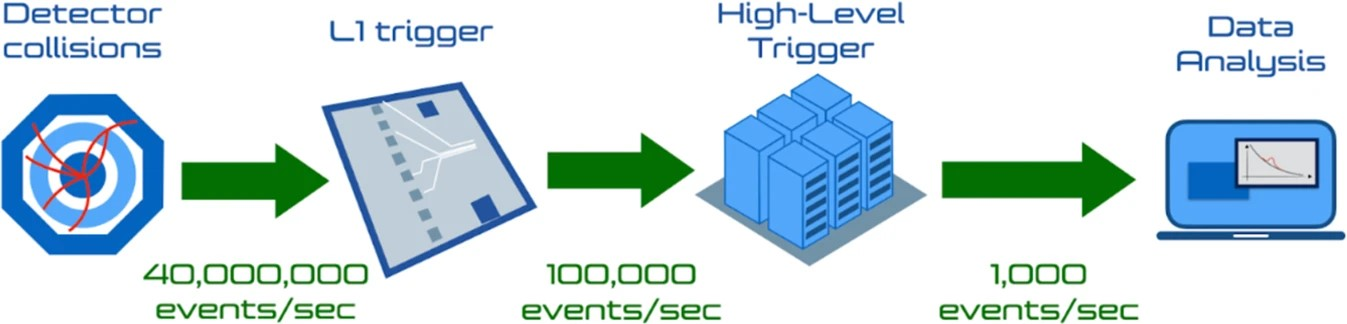
\includegraphics[width=0.8\linewidth]{Trigger_system.jpeg}
	\end{figure}

\end{frame}

\section{ML4DQM}
\begin{frame}
	\frametitle{Data Quality Monitoring}
	\begin{columns}
		\column{.4\linewidth}
		\begin{itemize}
			\item Two workflows --- Online and Offline
			      \begin{itemize}
				      \item Online -- Measure detector performance and raises alarm with low latency
				      \item Offline -- Bookkeping and data certification
			      \end{itemize}
			\item Goal is to minimize bad (low quality) data from reaching physics datasets
		\end{itemize}
		\column{.6\linewidth}
		\begin{figure}
			\centering
			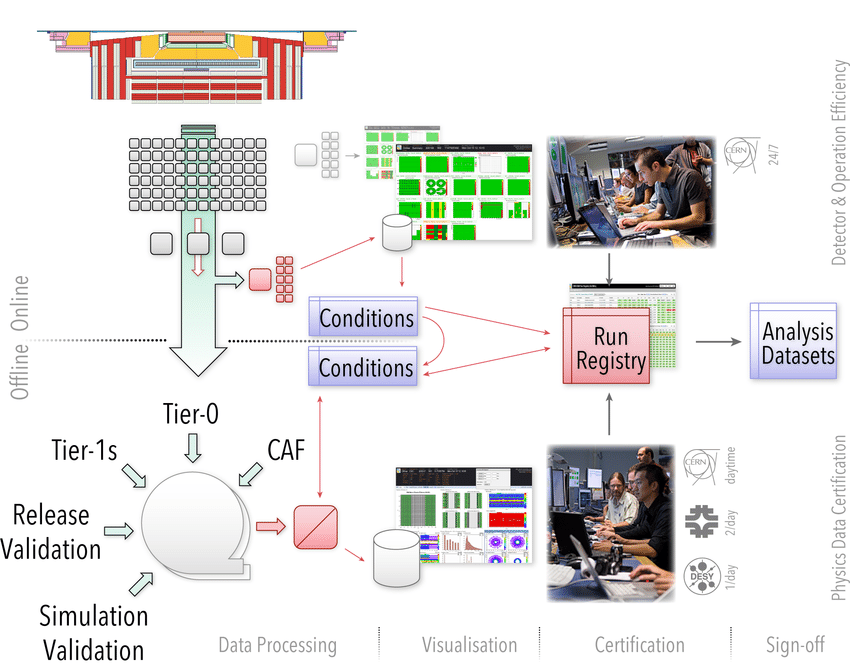
\includegraphics[width=\linewidth]{DQM Workflow.png}
		\end{figure}
	\end{columns}
\end{frame}
\begin{frame}
	\frametitle{DQM Shifts}
	\begin{itemize}
		\item Shifters are at the heart of this important process
		\item Labor intensive
		\item Lots of tools used to certify the data
		\item In the Upgraded detector, CMS Tracker alone will have 2 billion readout channels
		\item ML can help!
	\end{itemize}
	\begin{figure}
		\begin{center}
			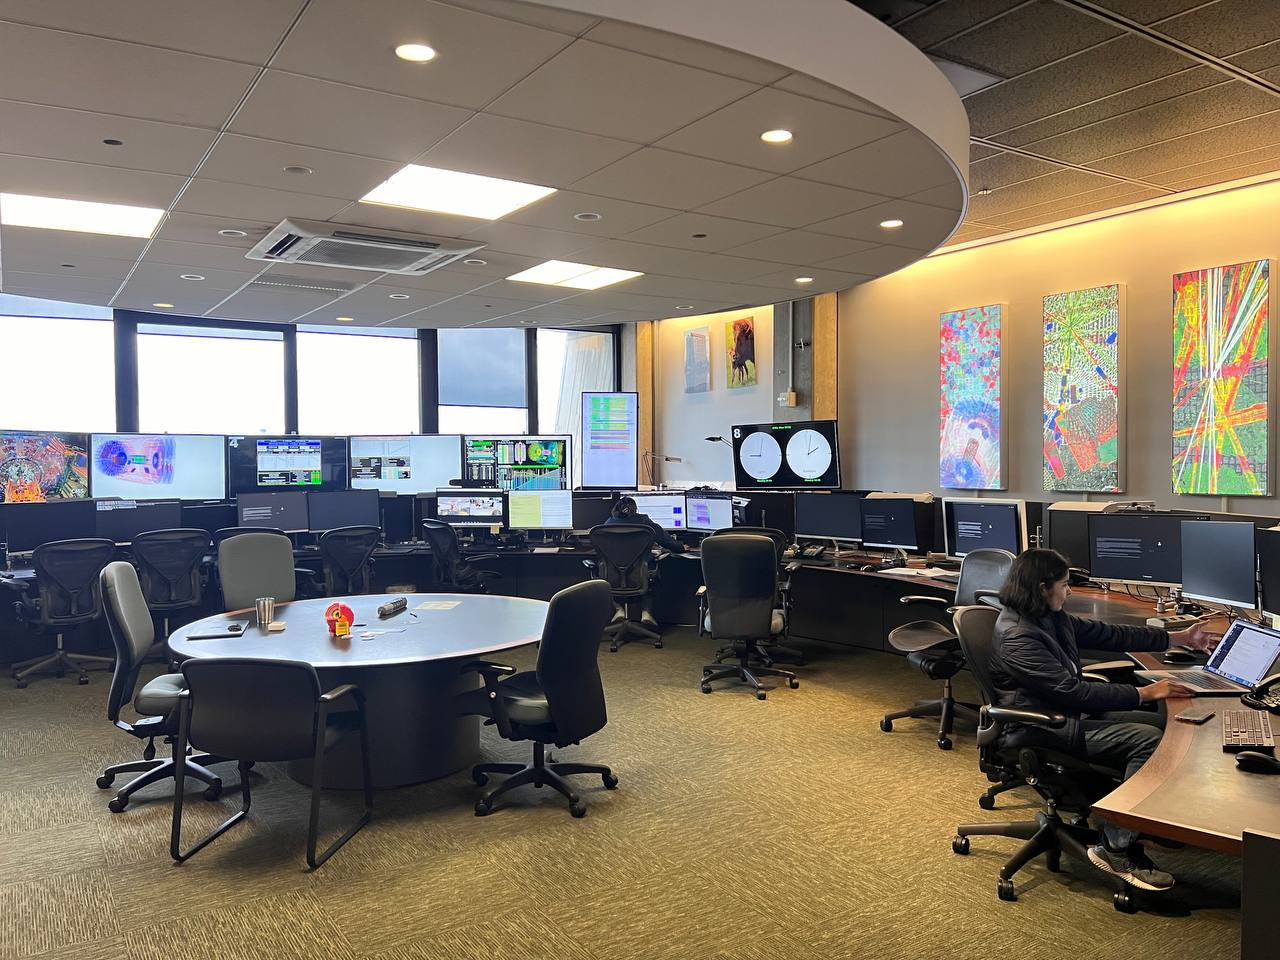
\includegraphics[width=.9\linewidth,trim=0 0 0 5.6in,clip ]{ROC_FNAL.jpg}
		\end{center}
	\end{figure}

\end{frame}

\begin{frame}
	\frametitle{ML4DQM}

	\begin{itemize}
		\item Assist to efficiently monitor and certify the current data via automation (of obvious cases)
		\item Campaigns for using more granular DQM data (lumisection level) potentially increases quantity of good data
		\item New challenges with HL-LHC upgrade (scale up)
		\item First we need to enable ML workflows
	\end{itemize}
	\begin{figure}
		\centering
		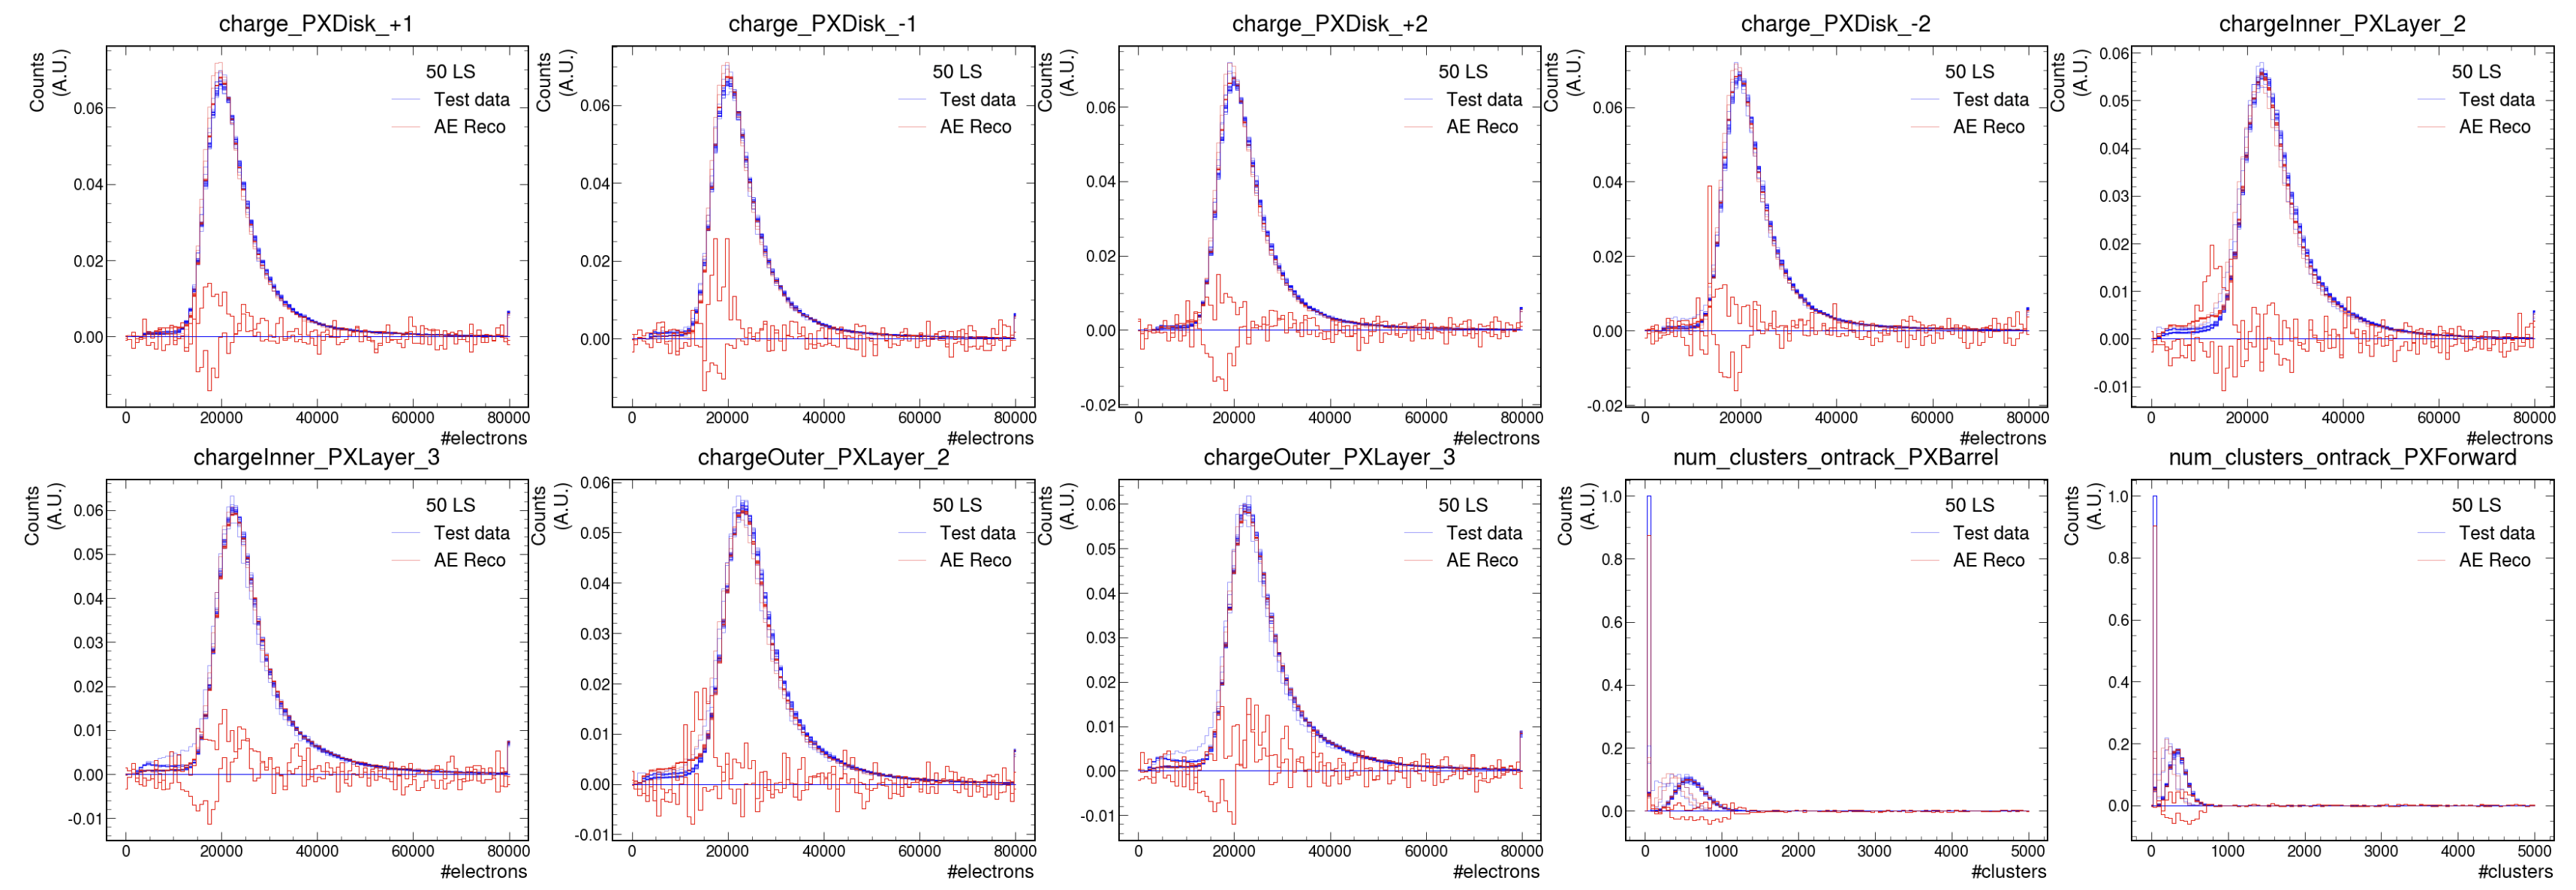
\includegraphics[width=\linewidth,trim = 0 4.1in 9.55in 0in, clip]{Project_Reco.png}
	\end{figure}

\end{frame}

\begin{frame}
	\frametitle{ML4DQM (Reference Run Ranking)}
	\begin{itemize}
		\item Assist shift leaders to efficiently select RRs
		\item Developed a python program that enables ranking based on data taking conditions
		\item This takes input from different DQM tools (RunRegistry and OMS)
		\item Can be used to provide input training dataset for ML models
	\end{itemize}
	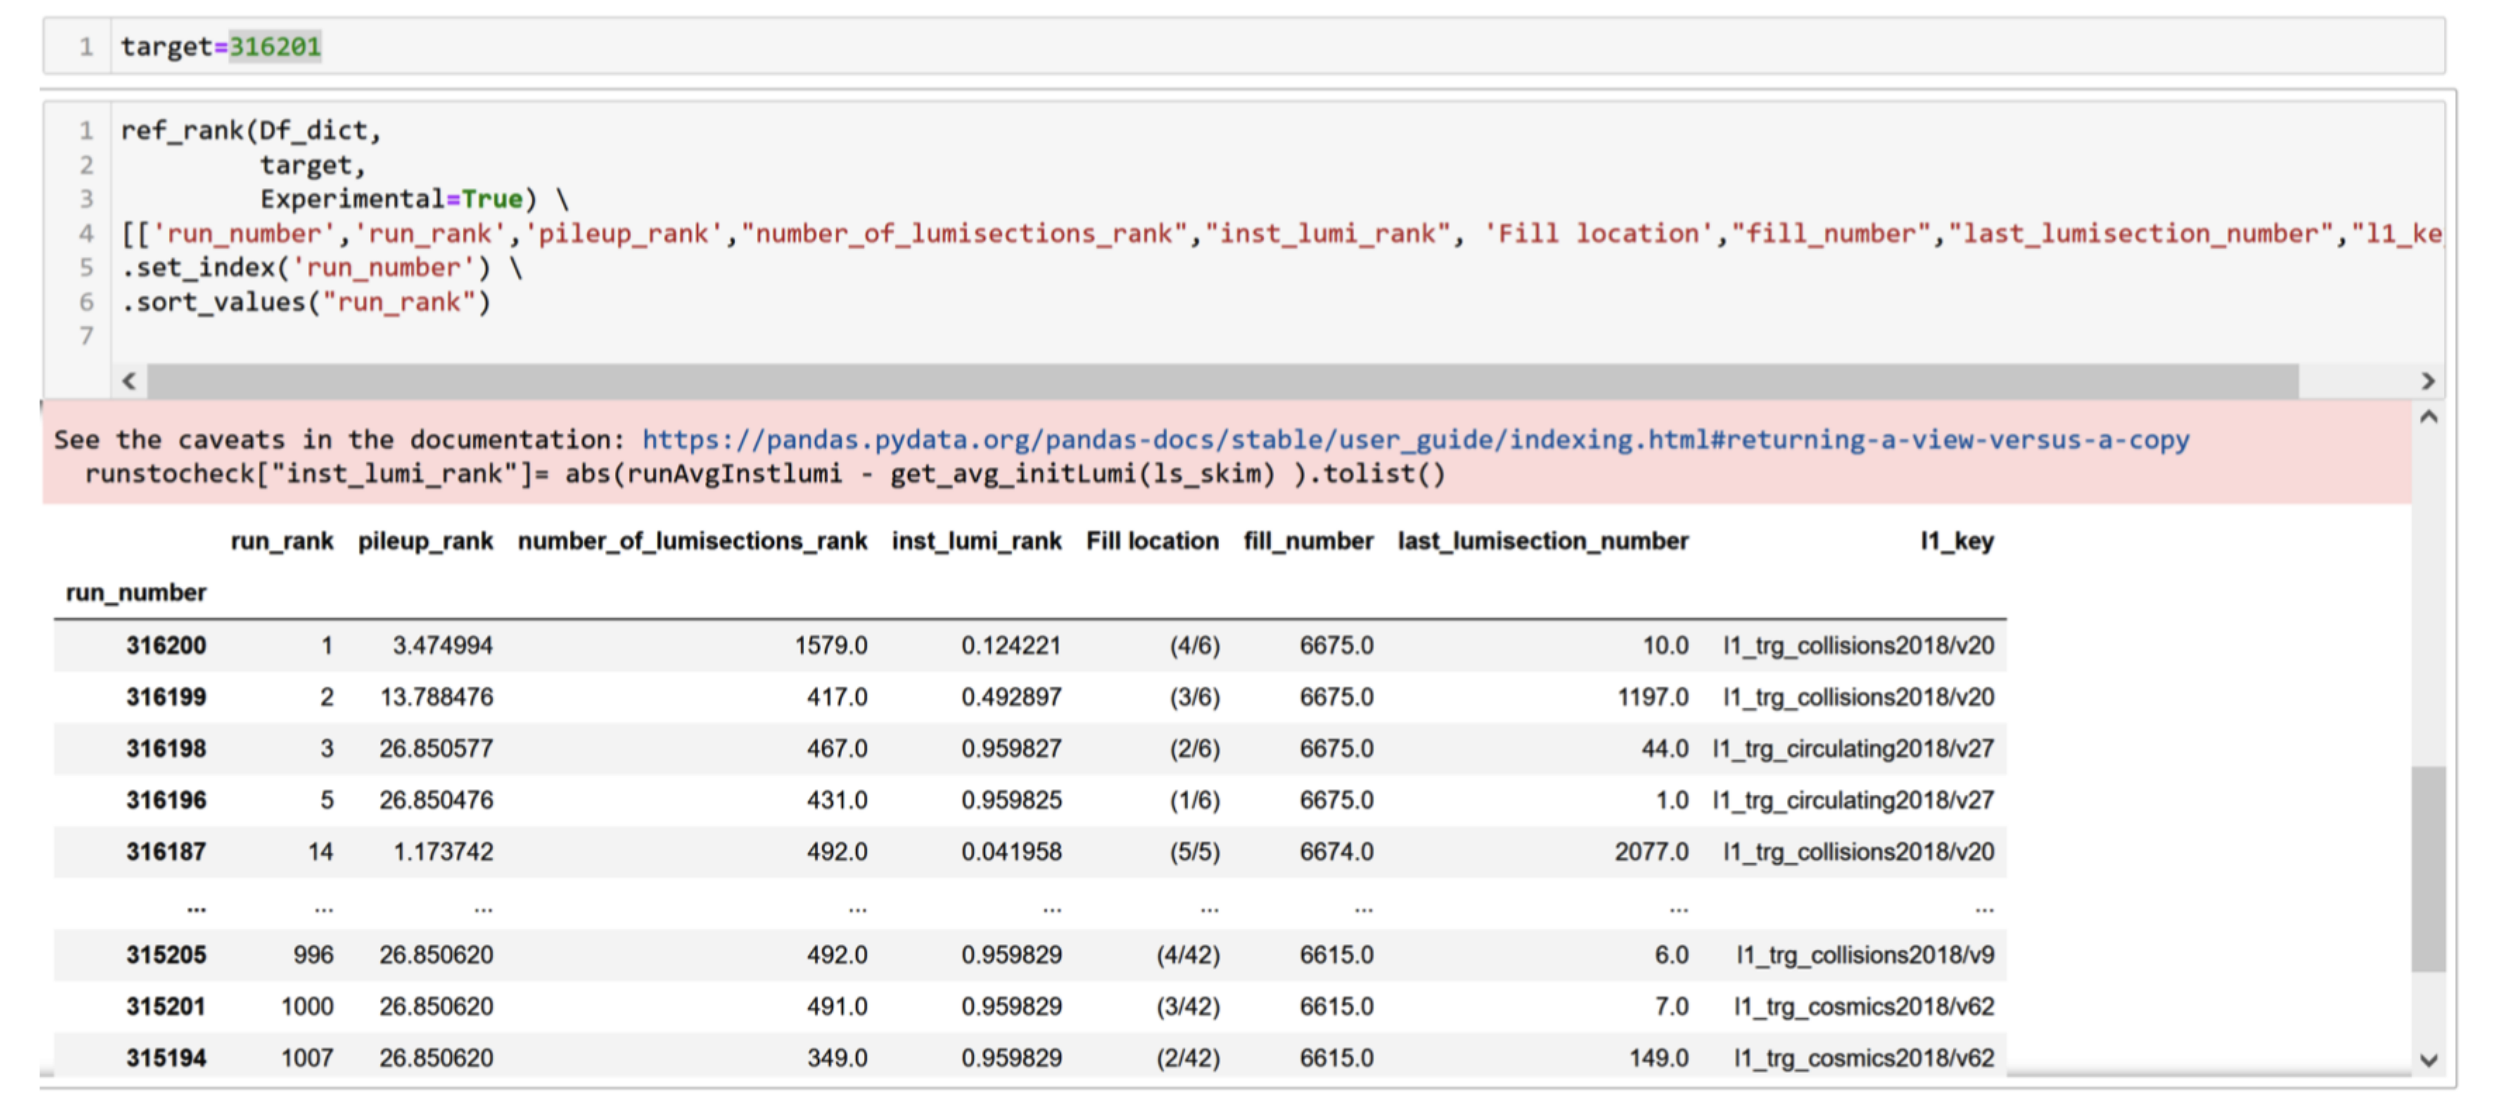
\includegraphics[width=\linewidth]{ranking.png}
\end{frame}

\begin{frame}
	\frametitle{ML4DQM (ML Playground)}
	\begin{itemize}
		\item Automated the ingestion of new data
		\item Can provide easier data exploration, input data and ML models
		\item All to provide good quality data for physics analyses
	\end{itemize}
	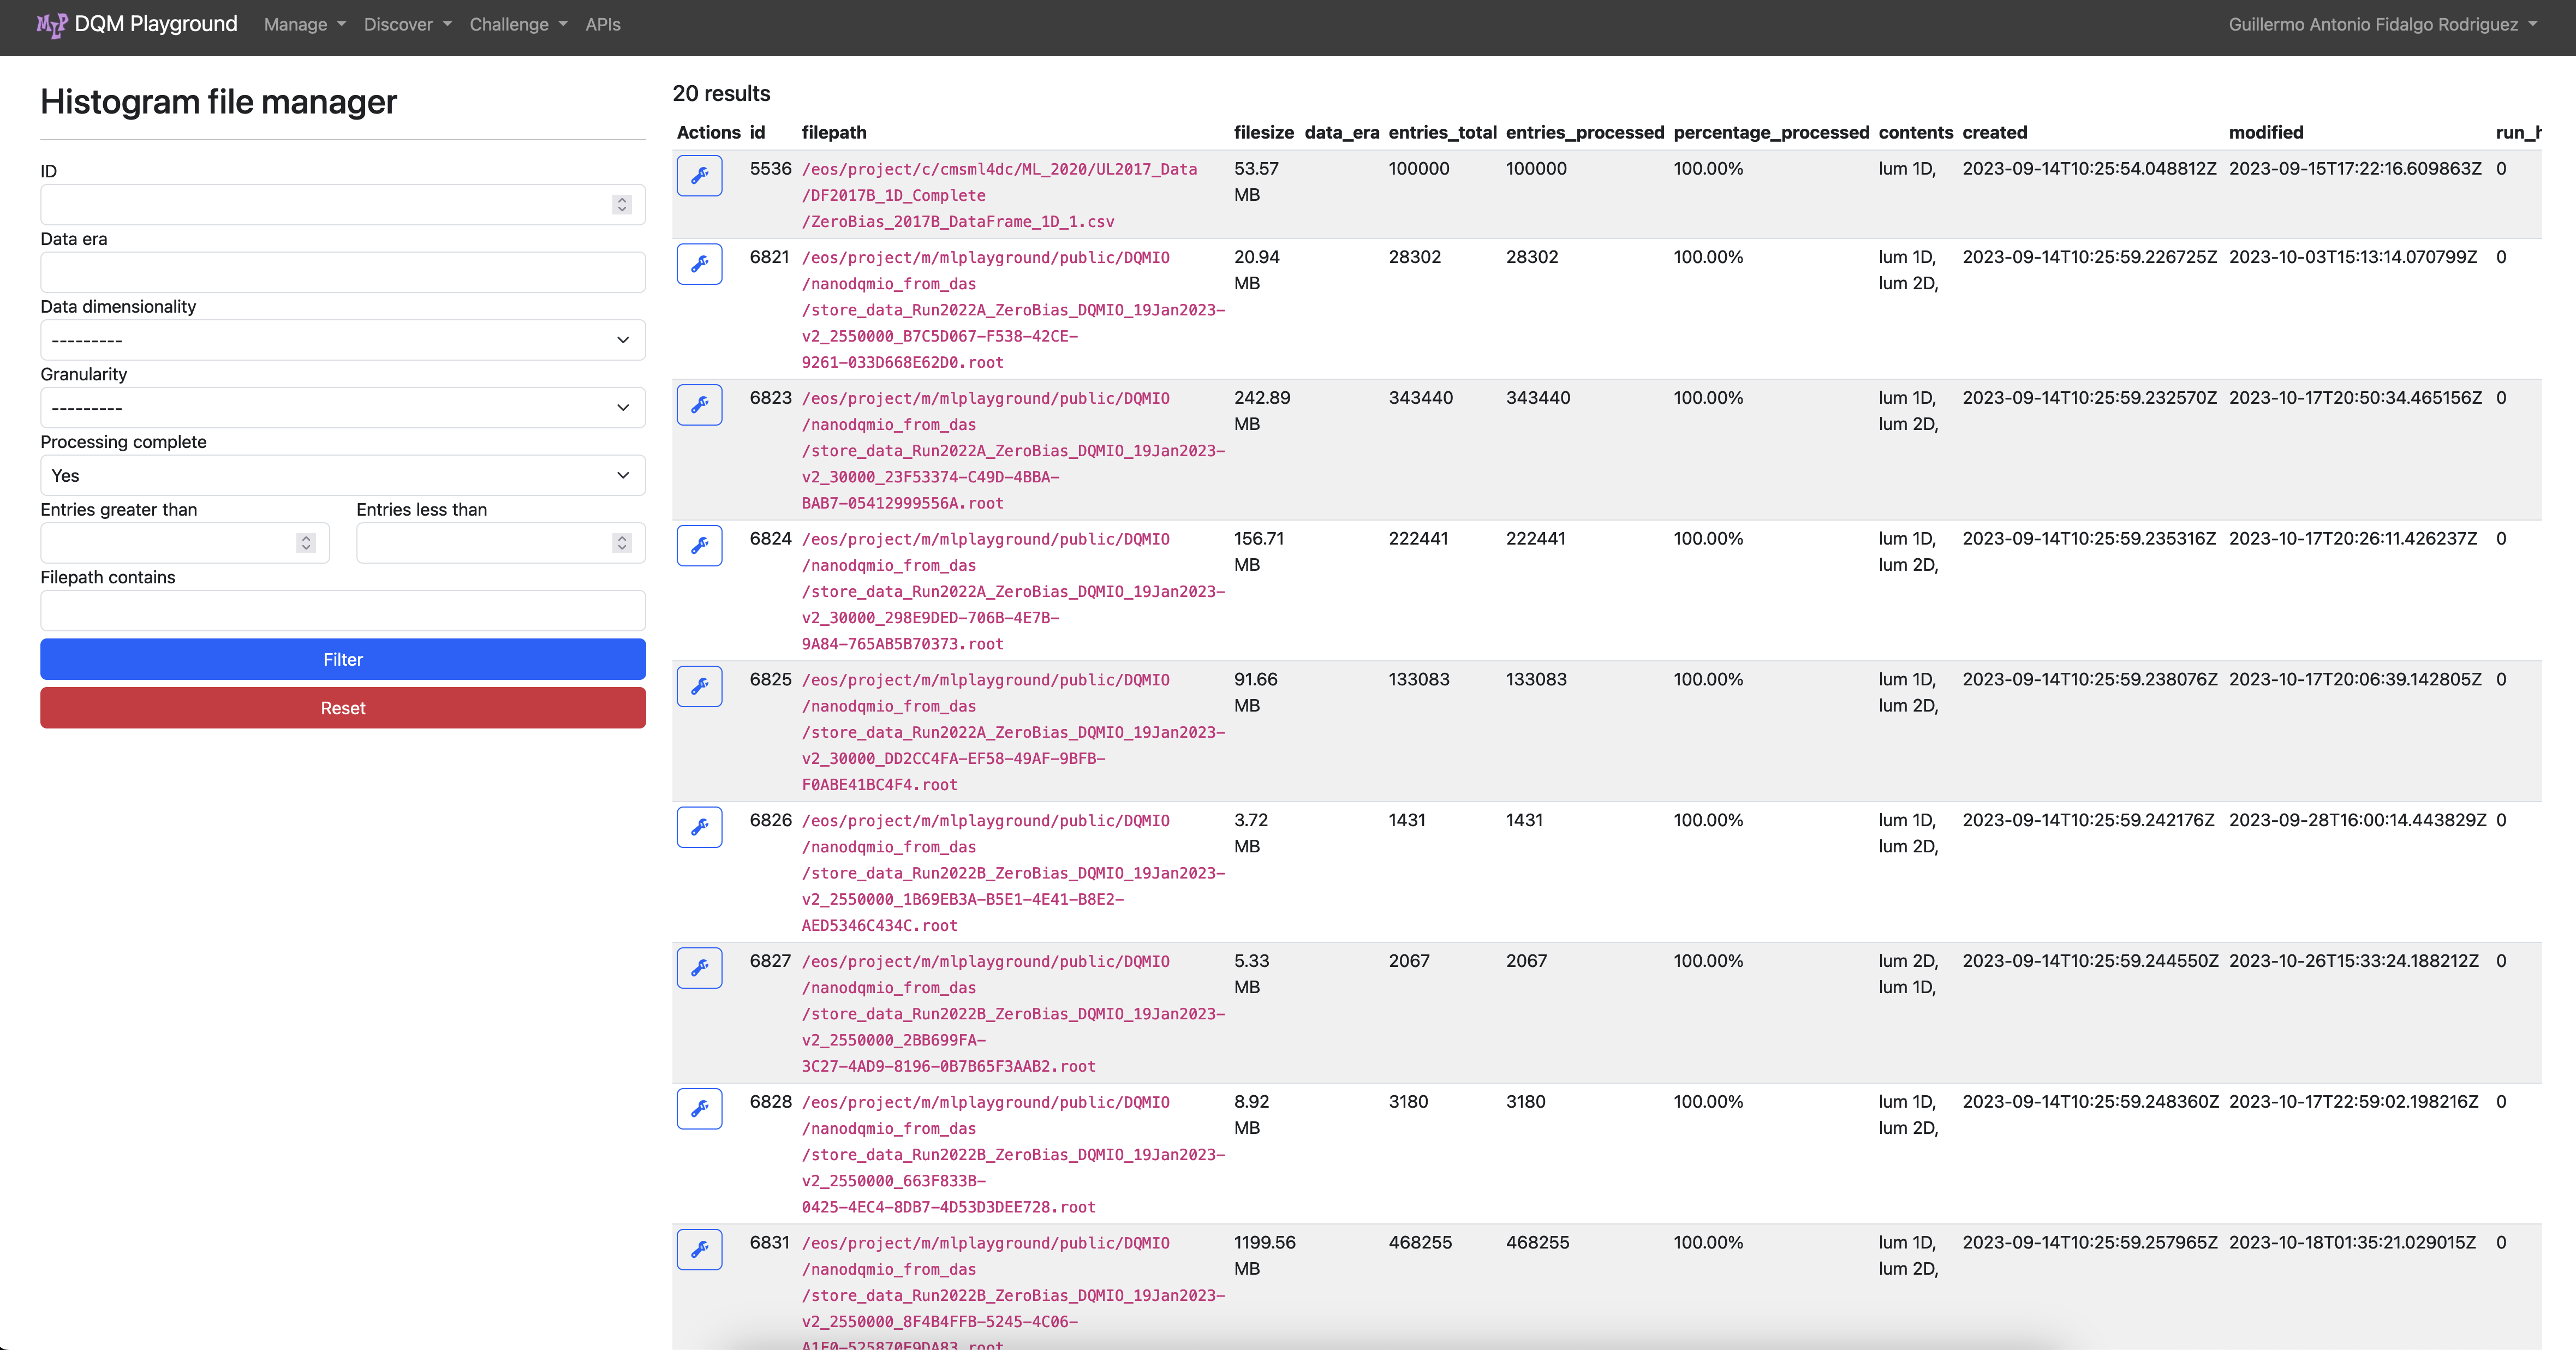
\includegraphics[width=\linewidth,trim= 0 7in 7in 0,clip]{MLP.png}
\end{frame}

\section{Emerging Jets Analysis}

\begin{frame}{Emerging Jets}
	\begin{columns}
		\column{.5\linewidth}
		\begin{itemize}
			\item Dark Matter model with a field analogous to QCD
			\item 2 phenomenological models -- Flavored (d,s,b) and Unflavored
			\item DM particles interact with SM through a dark mediator $X_{DK}$ and can be potentially produced at the LHC
		\end{itemize}
		\column{.5\linewidth}
		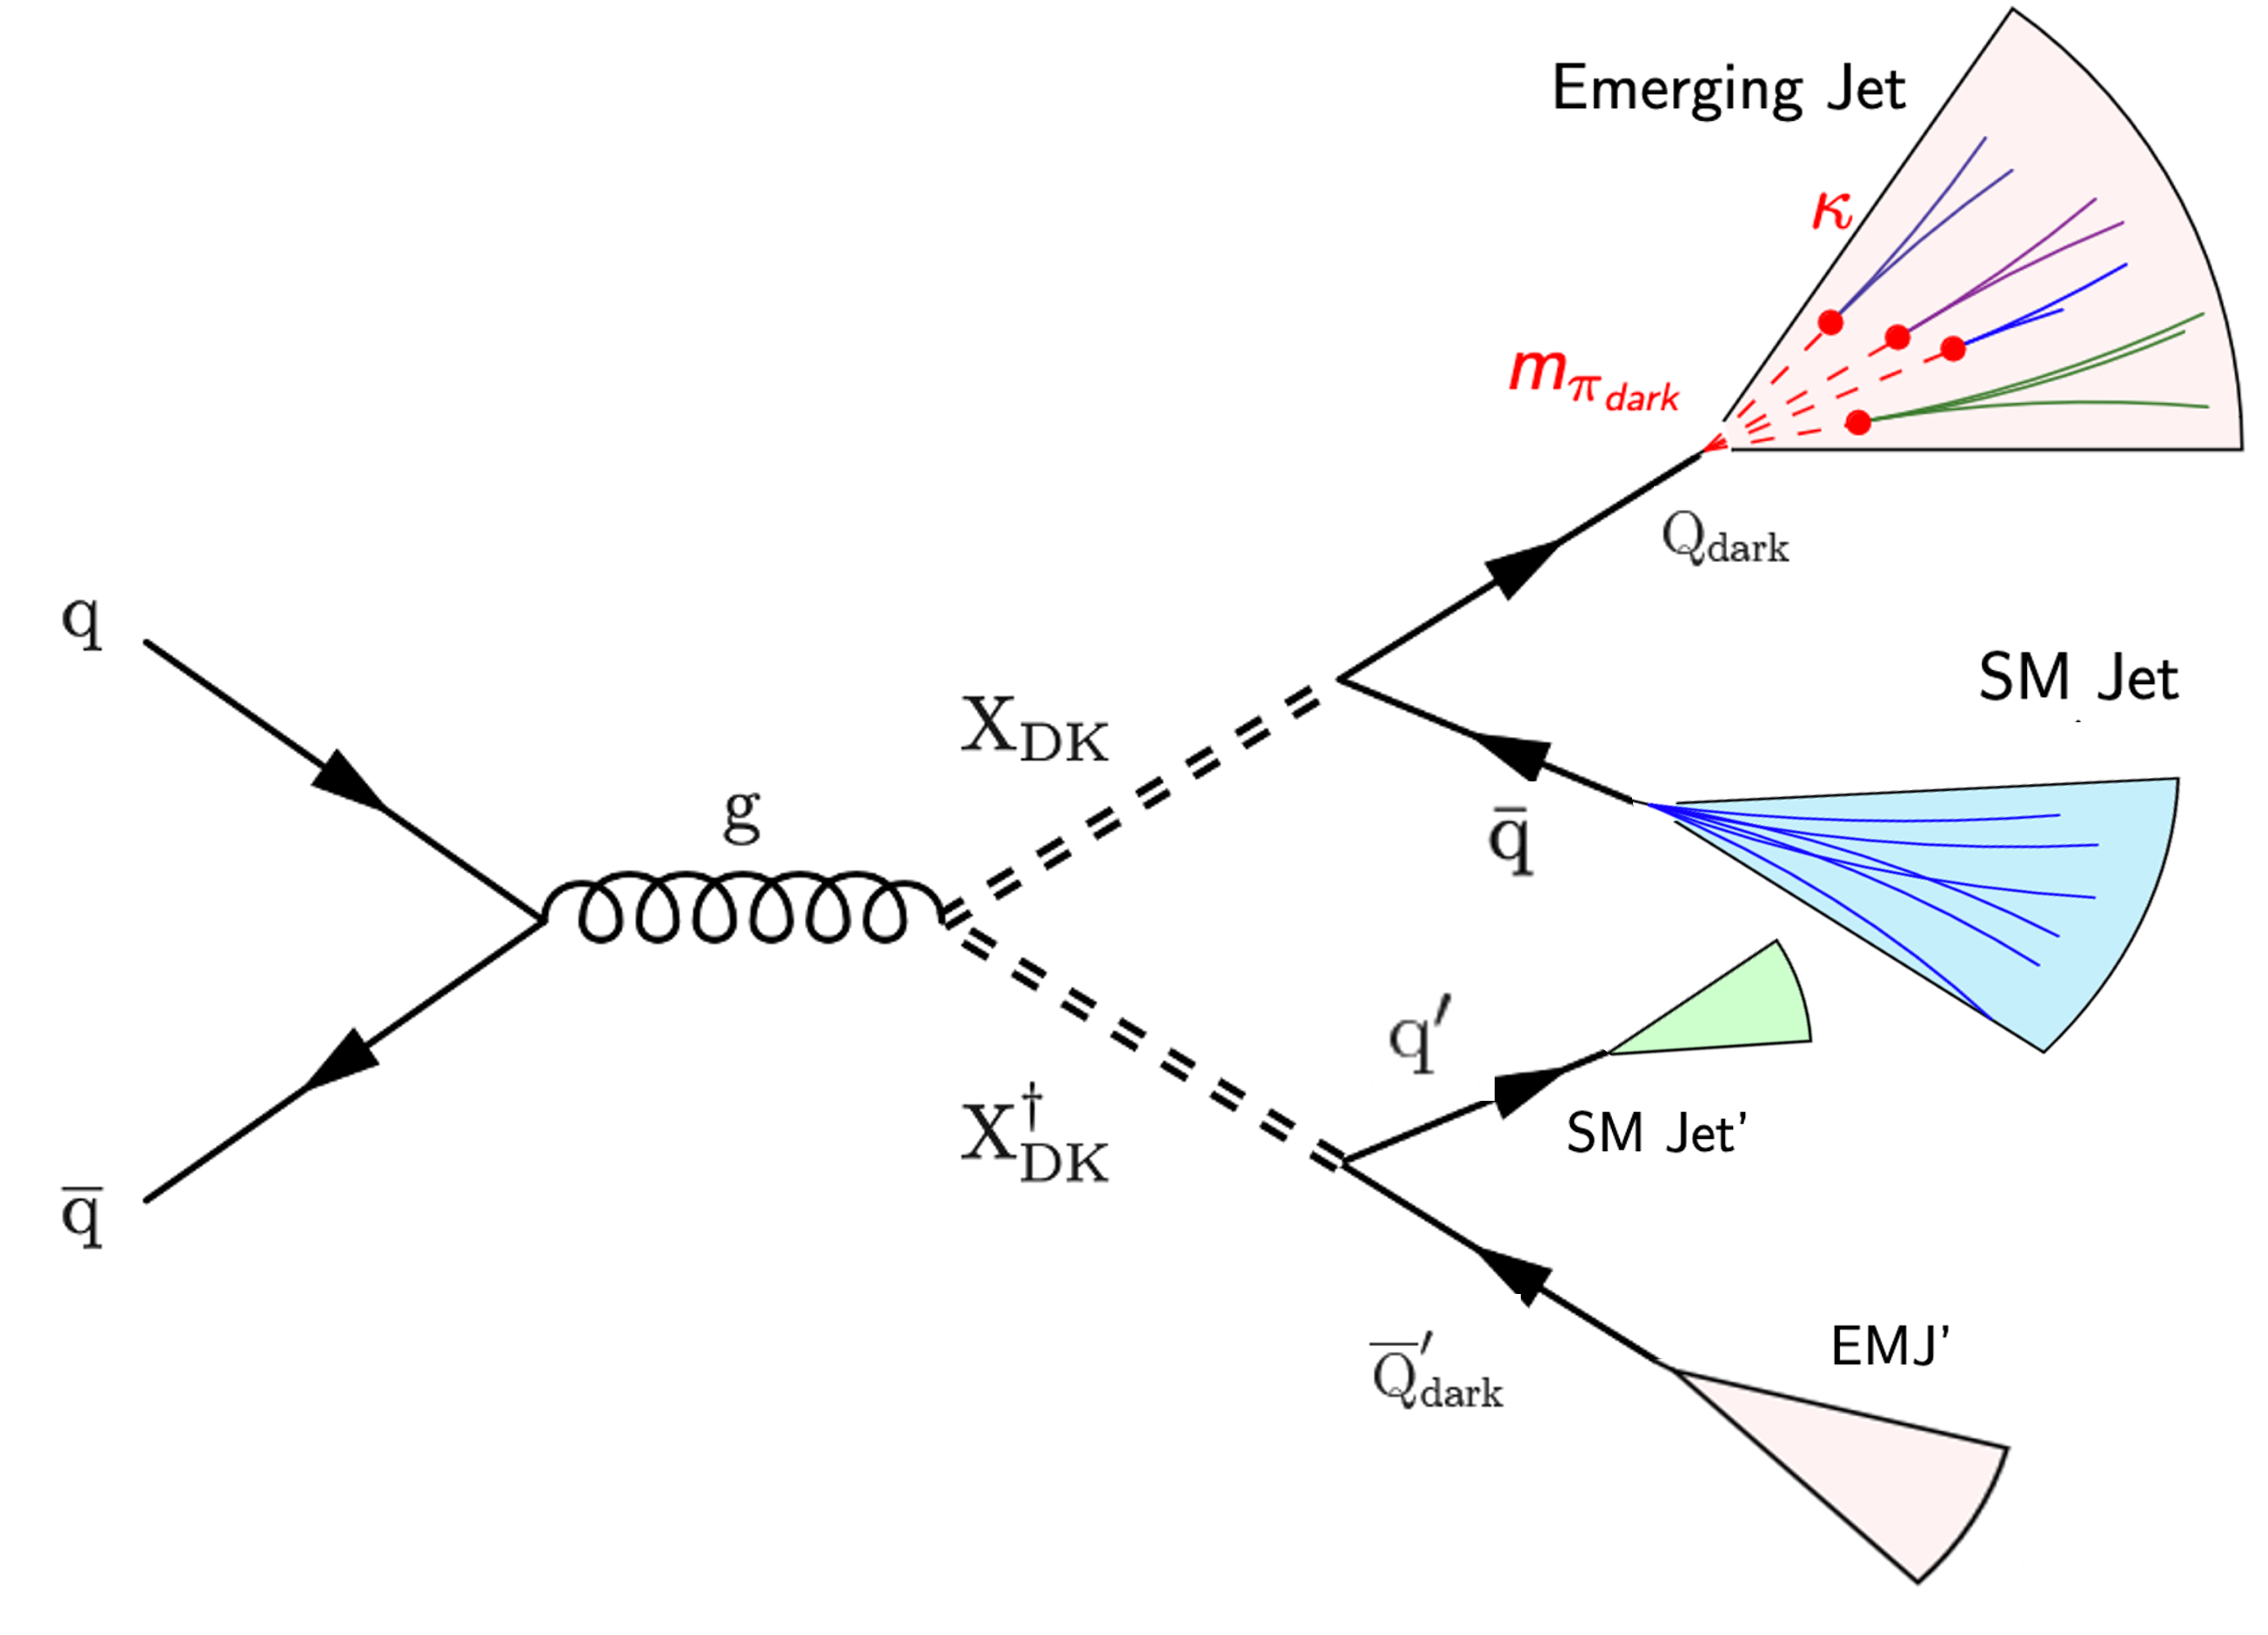
\includegraphics[width=\linewidth]{EMJ_production.png}
	\end{columns}
\end{frame}

\begin{frame}
	\frametitle{How do we search for EJs? (Event Selection)}
	\begin{columns}
		\column{.6\linewidth}
		\begin{itemize}
			\item High $H_T$
			\item 4 high $p_T$ jets (2 EJs and 2 SM Jets)
			\item Scan parameter space:
			      \begin{itemize}
				      \item $m_{X_{DK}} \in [1,2.5] $ TeV
				      \item $m_{\pi_{DK}} \leq 20$ GeV
				      \item $c\tau_{\pi_{DK}} \leq 500$ mm
			      \end{itemize}
		\end{itemize}

		\begin{figure}
			\centering
			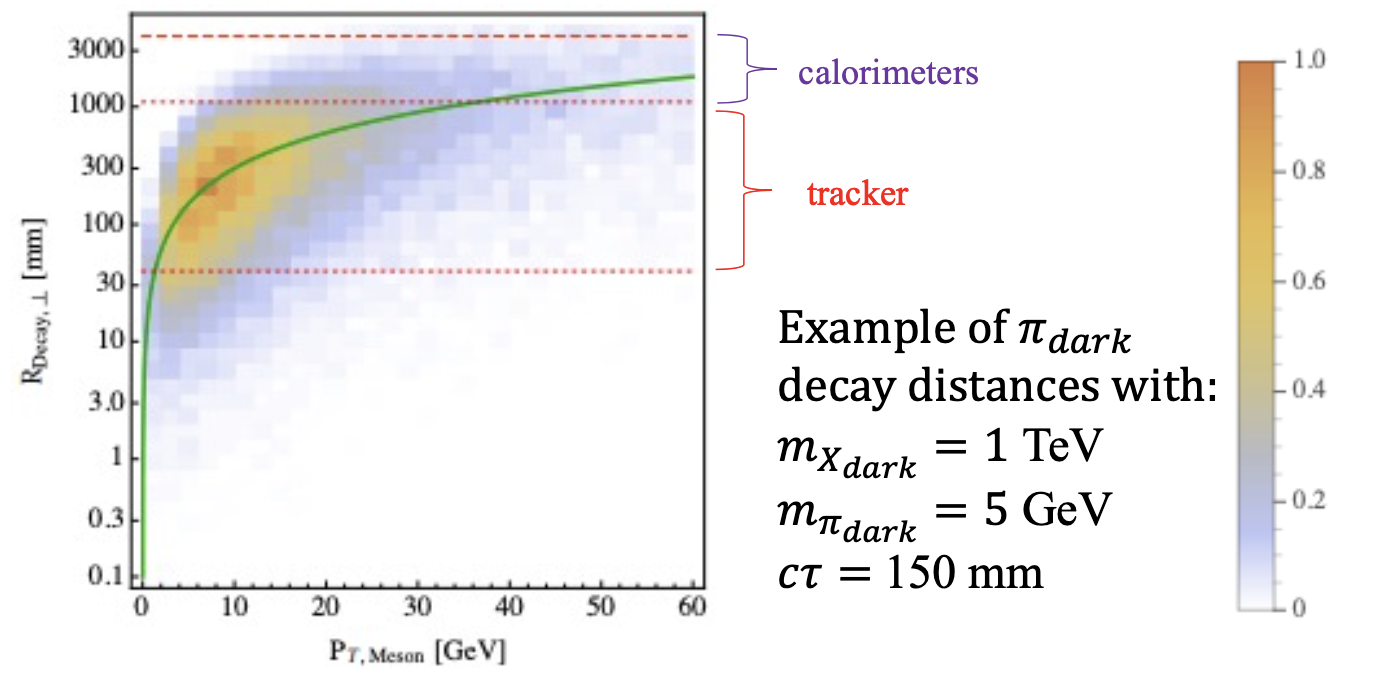
\includegraphics[width=\linewidth]{Decay-distances-emj.png}
		\end{figure}

		\column{.4\linewidth}

		\begin{figure}
			\centering
			\includegraphics[width=.9\linewidth]{emj_detector.png}
		\end{figure}


	\end{columns}

\end{frame}


\begin{frame}
	\frametitle{Results of the analysis}
	\begin{itemize}
		\item Despite the amount of data collected and the improved methods used for the analysis (EJs ML Tagger) we did not see a significant deviation in the signal over the background
		\item We impose limits with 95\% upper CL that can be found in the \href{https://doi.org/10.48550/arXiv.2403.01556}{paper}

		\item For the unflavored model, $m_{X_{DK}} <$  1950 GeV are excluded for $c\tau_{\pi_{DK}} \approx$ 100mm and $m_{\pi_{DK}}=$~10~GeV

		\item  The flavor-aligned excludes $m_{X_{DK}} <$  1850 GeV at $c\tau^{max}_{\pi_{DK}} \approx$ 500mm for
		      $m_{\pi_{DK}}$= 10GeV

		\item This result surpasses the previous search for emerging jets in the unflavored scenario, and increases the limit of the dark mediator particle by $\approx$ 500GeV
	\end{itemize}


\end{frame}


\begin{frame}
	\frametitle{My contributions: Trigger Efficiency Studies}
	\begin{itemize}
		% \item Triggers are first step to generating datasets required for physics analyses
		\item Select 2 data streams and modeled their efficiency
		\item Lowest $H_T$ (or $p_T$) unpre-scaled trigger
		      % \item Impose relevant conditions for each analysis on top of the Trigger selections to measure efficiency
	\end{itemize}

	\begin{columns}
		\column{.4\linewidth}
		\begin{figure}
			\centering
			\includegraphics<1>[width=\linewidth]{pdfs/18_efficiency_withratio_and_fits.pdf}
			\includegraphics<2>[width=\linewidth]{pdfs/18_SinglePhoton_efficiency_withratio_and_fits.pdf}
		\end{figure}

		\column{.6\linewidth}

		\begin{align}
			\text{erf}(H_T ;\ A,B,C) & = \frac{A}{2} \left[1+ \text{erf}\left(\dfrac{H_T - |B|}{C}\right) \right] \\
			f(H_T ;\ A,B,C,D)        & = A \dfrac{\frac{H_T - B}{C}}{1+ \left(\frac{H_T - B}{C}\right)^2} + D
		\end{align}

	\end{columns}

\end{frame}


\section{Summary}

\begin{frame}
	\frametitle{Summary}
	\begin{itemize}
		\item At the LHC, physicists are looking for Physics discoveries beyond the SM via high-energy collisions
		\item ML4DQM is an important workflow responsible of providing CMS high-quality data and ML can provide improvements
		\item Work is underway to provide a platform for ML development and ML4DQM studies
		\item CMS is potentially sensitive to proposed dark matter models like EJs and new limits were set on this model
		\item Trigger studies were performed for the EJs analysis and this work is to be published soon in JHEP.
	\end{itemize}

\end{frame}

\begin{frame}{Semester Abroad and Presentations at FNAL and CERN, Switzerland}
	\begin{figure}
		\centering
		\begin{subfigure}[t]{.9\linewidth}
			\centering
			\caption*{Semester at CERN}
			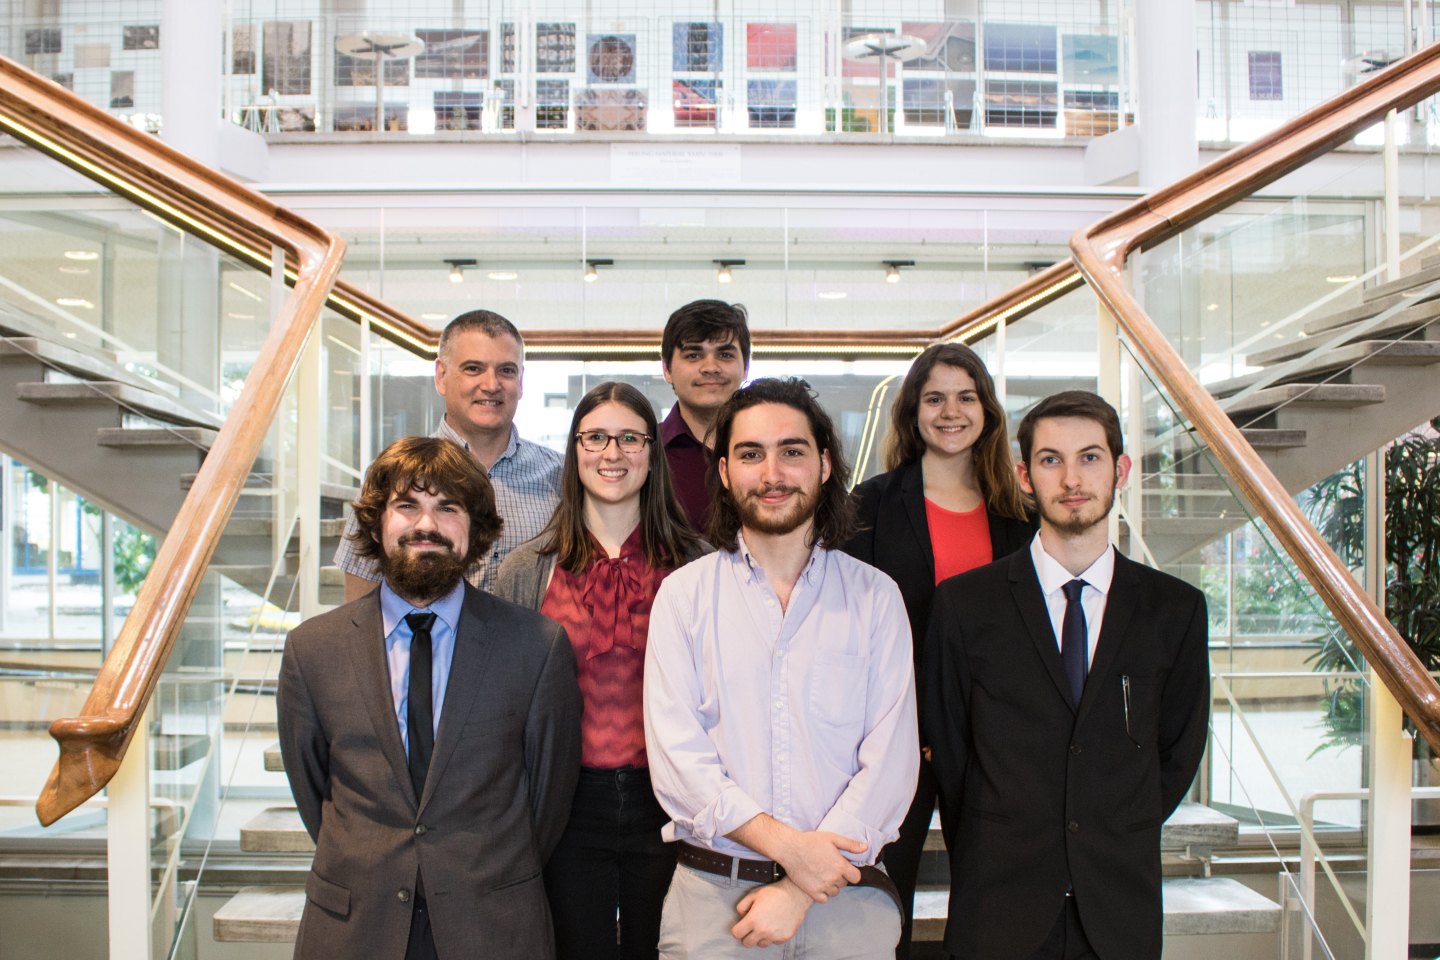
\includegraphics[width=.3\linewidth]{Collage/Group1.jpg}
			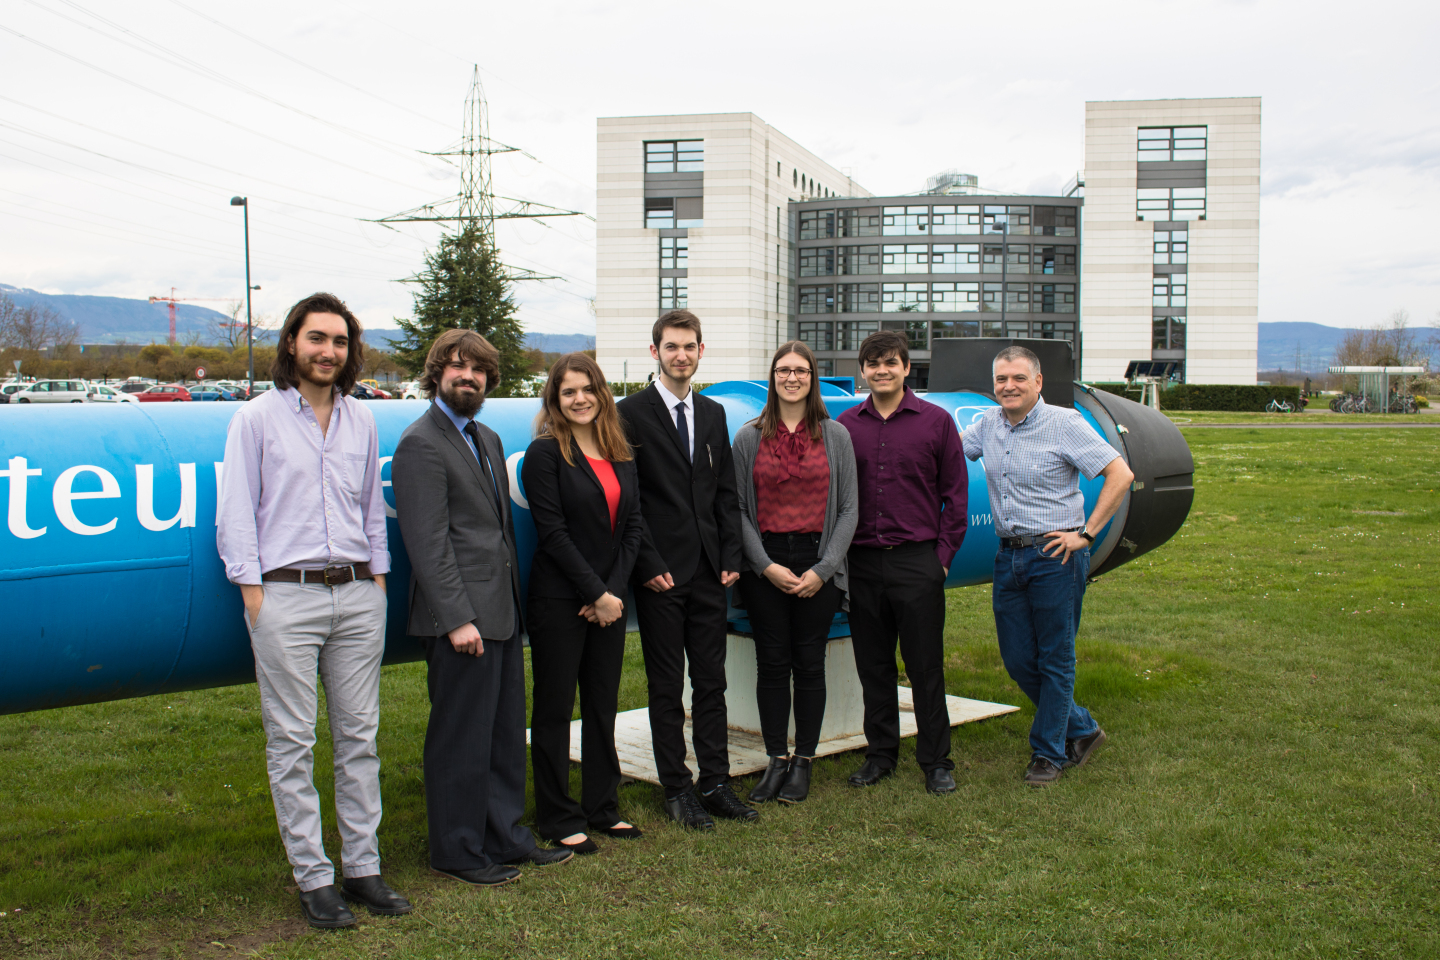
\includegraphics[width=.3\linewidth]{Collage/Group2.jpg}
			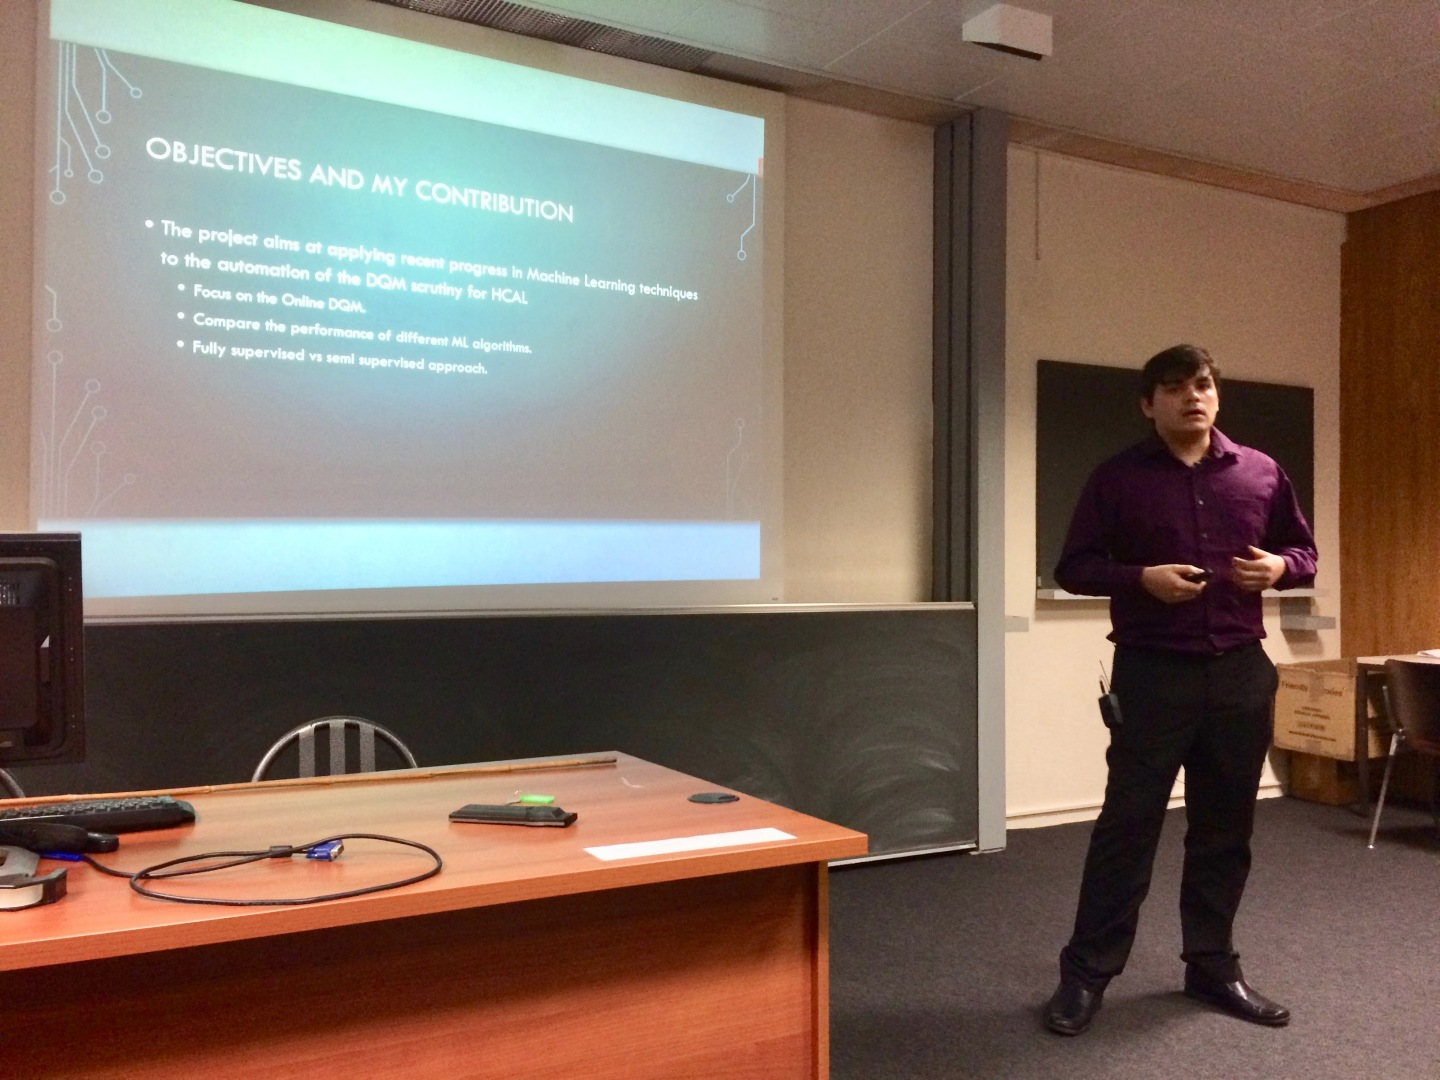
\includegraphics[width=.3\linewidth]{Collage/GuillermoFidalgoRodriguez.jpg}
		\end{subfigure}

		\begin{subfigure}[b]{.9\linewidth}
			\centering
			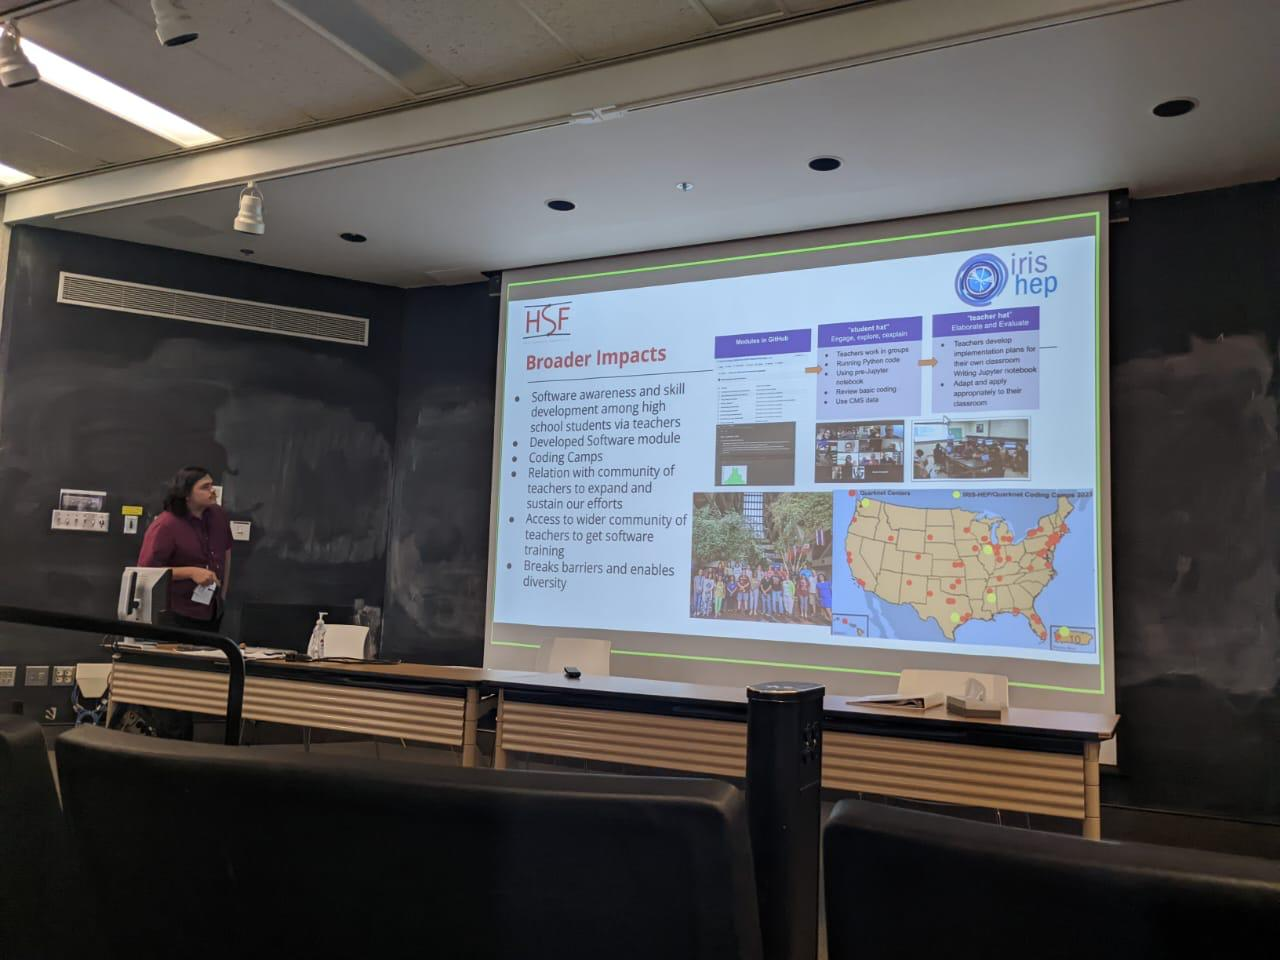
\includegraphics[width=.3\linewidth]{Collage/Guillermo_Talk1.jpg}
			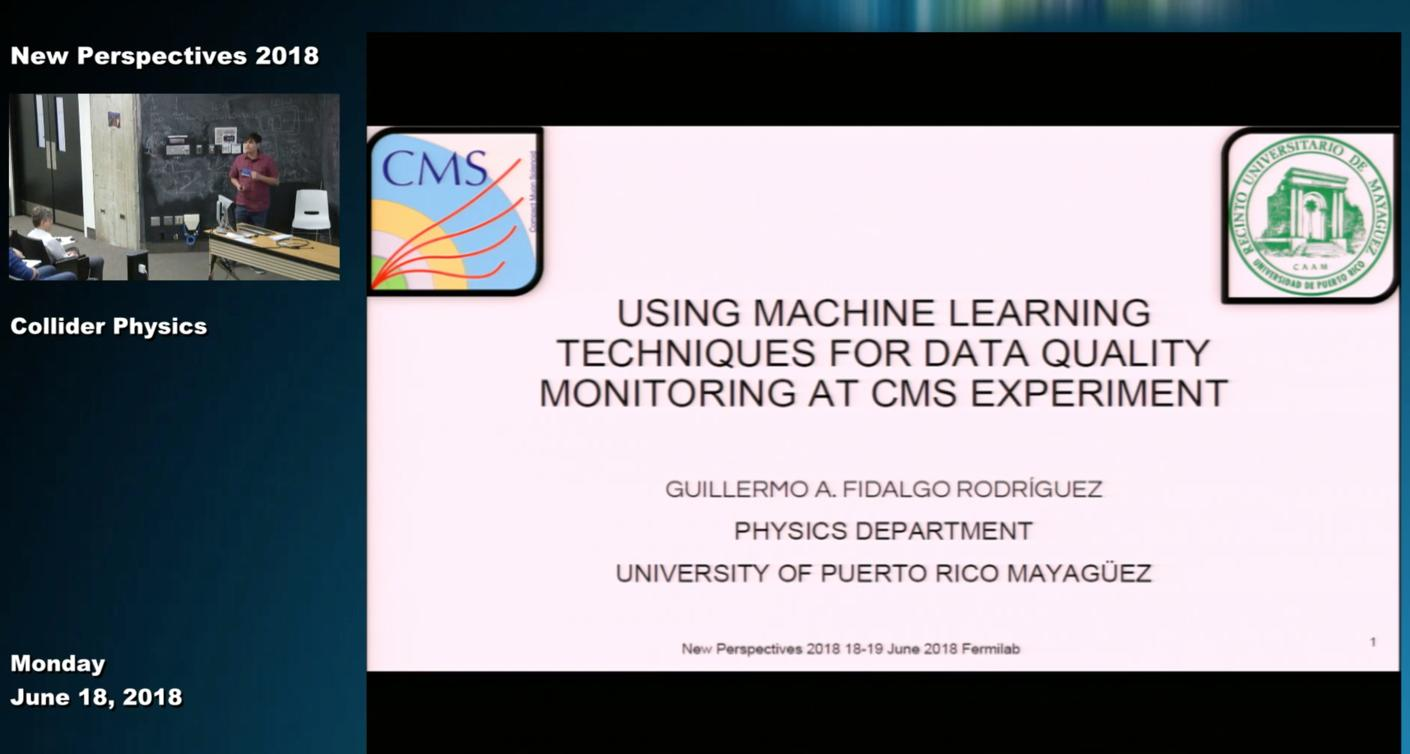
\includegraphics[width=.3\linewidth,trim= 0 6.2in 15in 1cm, clip]{Collage/Guillermo_Talk3.jpg}
			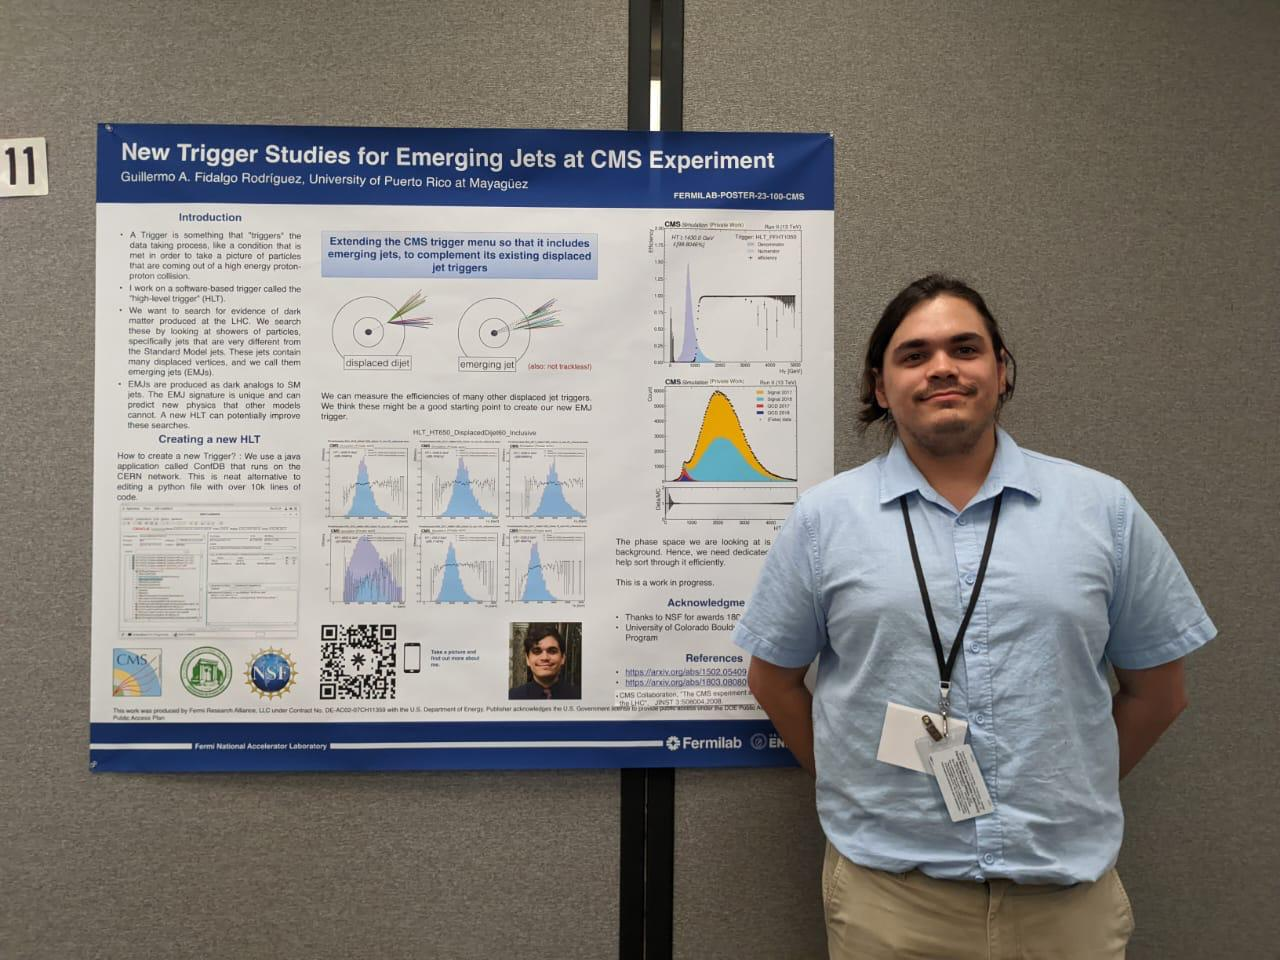
\includegraphics[width=.3\linewidth]{Collage/Guillermo_Talk2.jpg}
			\caption*{New Perspectives / USCMS Users Meeting}
		\end{subfigure}
	\end{figure}
\end{frame}



\begin{frame}
	\frametitle{Acknowledgments}

	\begin{itemize}
		\item Thanks for everyone in the EJs analysis group
		\item The LPC scientists
		\item UPRM Physics Dept.
		\item Prof. Sudhir Malik
		\item NSF Grant PHY-2111134
		\item Many, many more \dots
	\end{itemize}



\end{frame}

\begin{frame}
	\begin{center}
		{\Huge Thank you.\\ \vspace{1cm} Any Questions?}
	\end{center}
\end{frame}


%%%% Copy all this together %%%%%

\appendix

\section{Backup}

\begin{frame}
	\begin{center}
		{\Huge Backup}
	\end{center}
\end{frame}
%%%%%%%%%%%%%%%%%%%%%%%%%%%%%%%

\begin{frame}
	\frametitle{Pictures}
	\begin{figure}
		\centering
		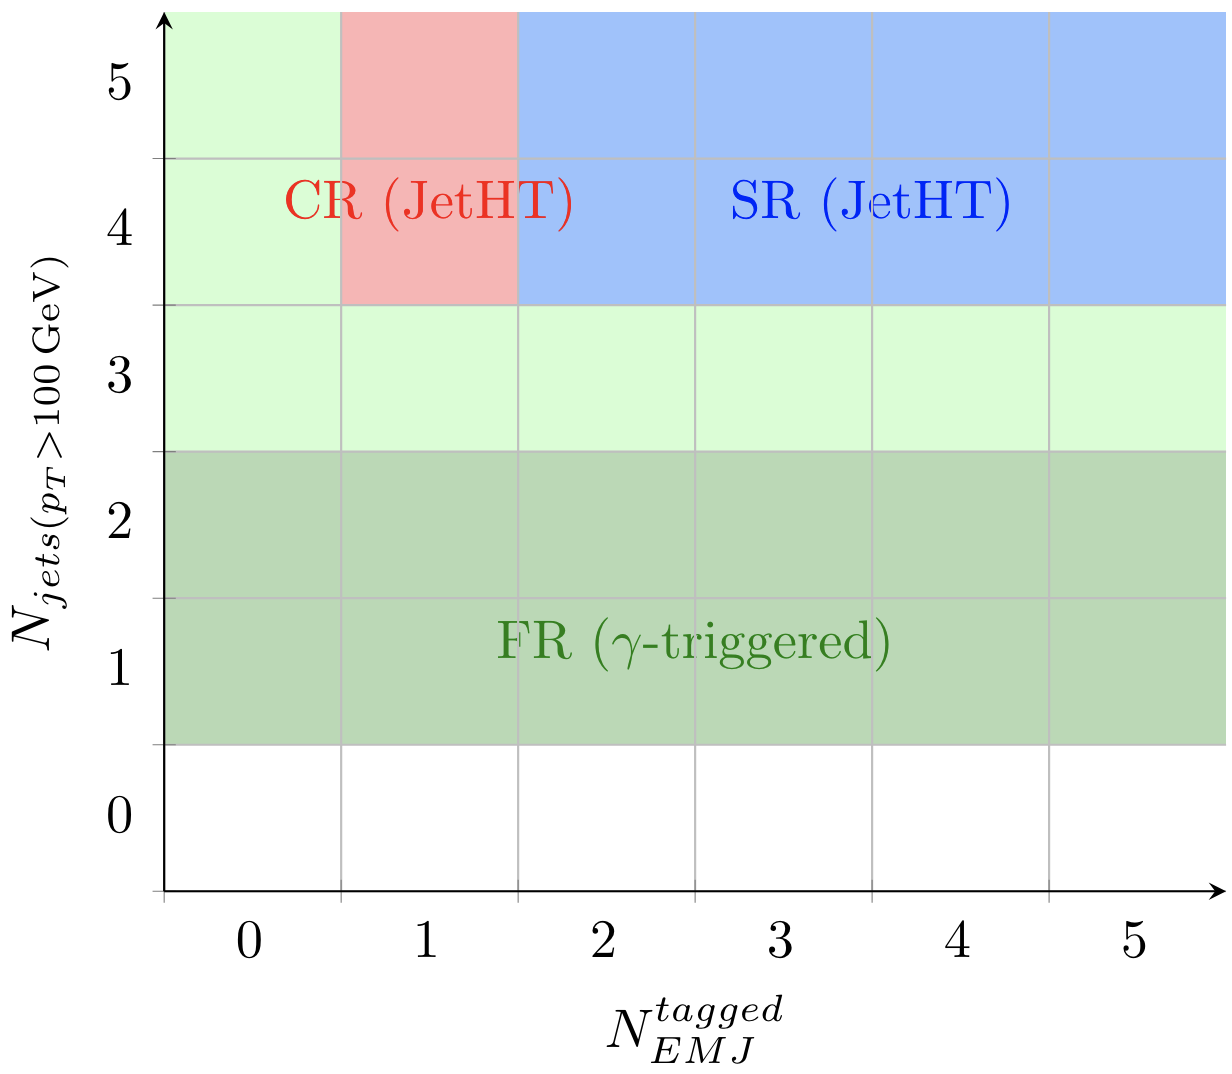
\includegraphics[height=.8\paperheight]{Regions.png}
	\end{figure}
\end{frame}

\begin{frame}
	\frametitle{More pictures}
	\begin{figure}
		\begin{subfigure}{.32\linewidth}
			\centering
			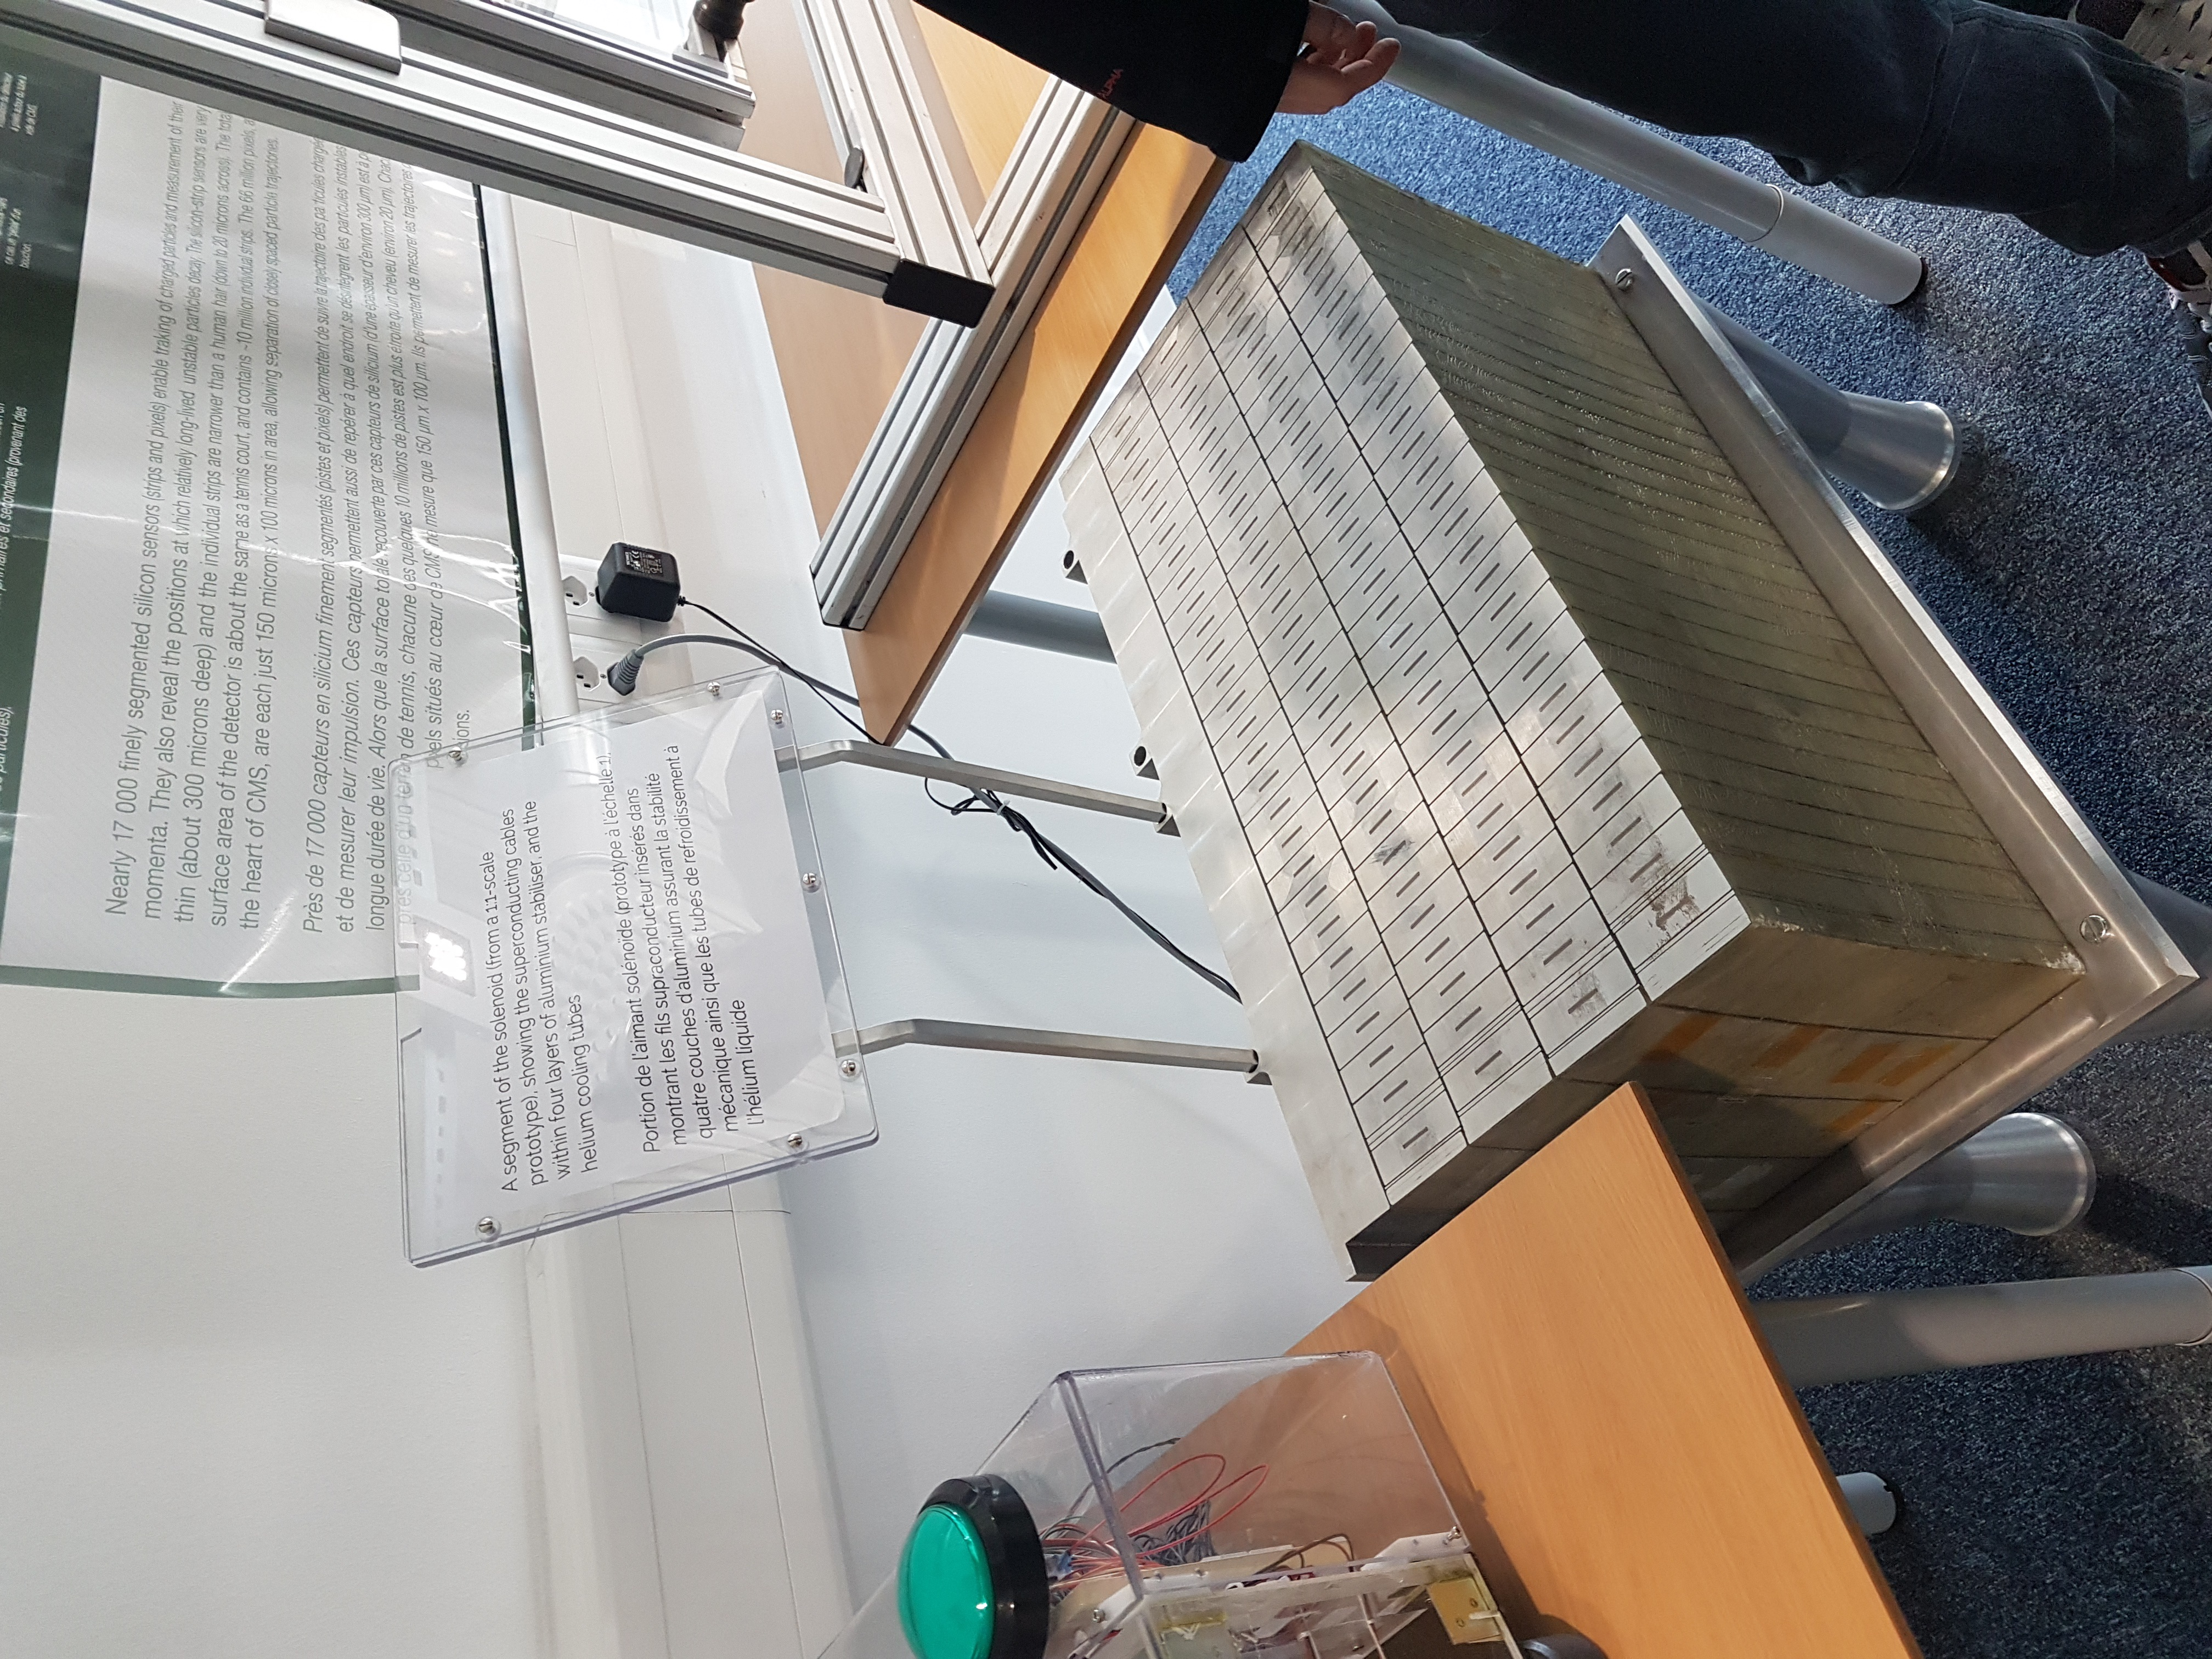
\includegraphics[width=6cm, angle=270]{Solenoid_piece.jpeg}
		\end{subfigure}
		\begin{subfigure}{.32\linewidth}
			\centering
			\includegraphics[width=6cm, angle=270]{HLT_farm.jpg}
		\end{subfigure}
		\begin{subfigure}{.32\linewidth}
			\centering
			\includegraphics[width=6cm, angle=90]{Me_at_CMS.jpg}
		\end{subfigure}
	\end{figure}
\end{frame}

\begin{frame}{ML4DQM}
	\centering
	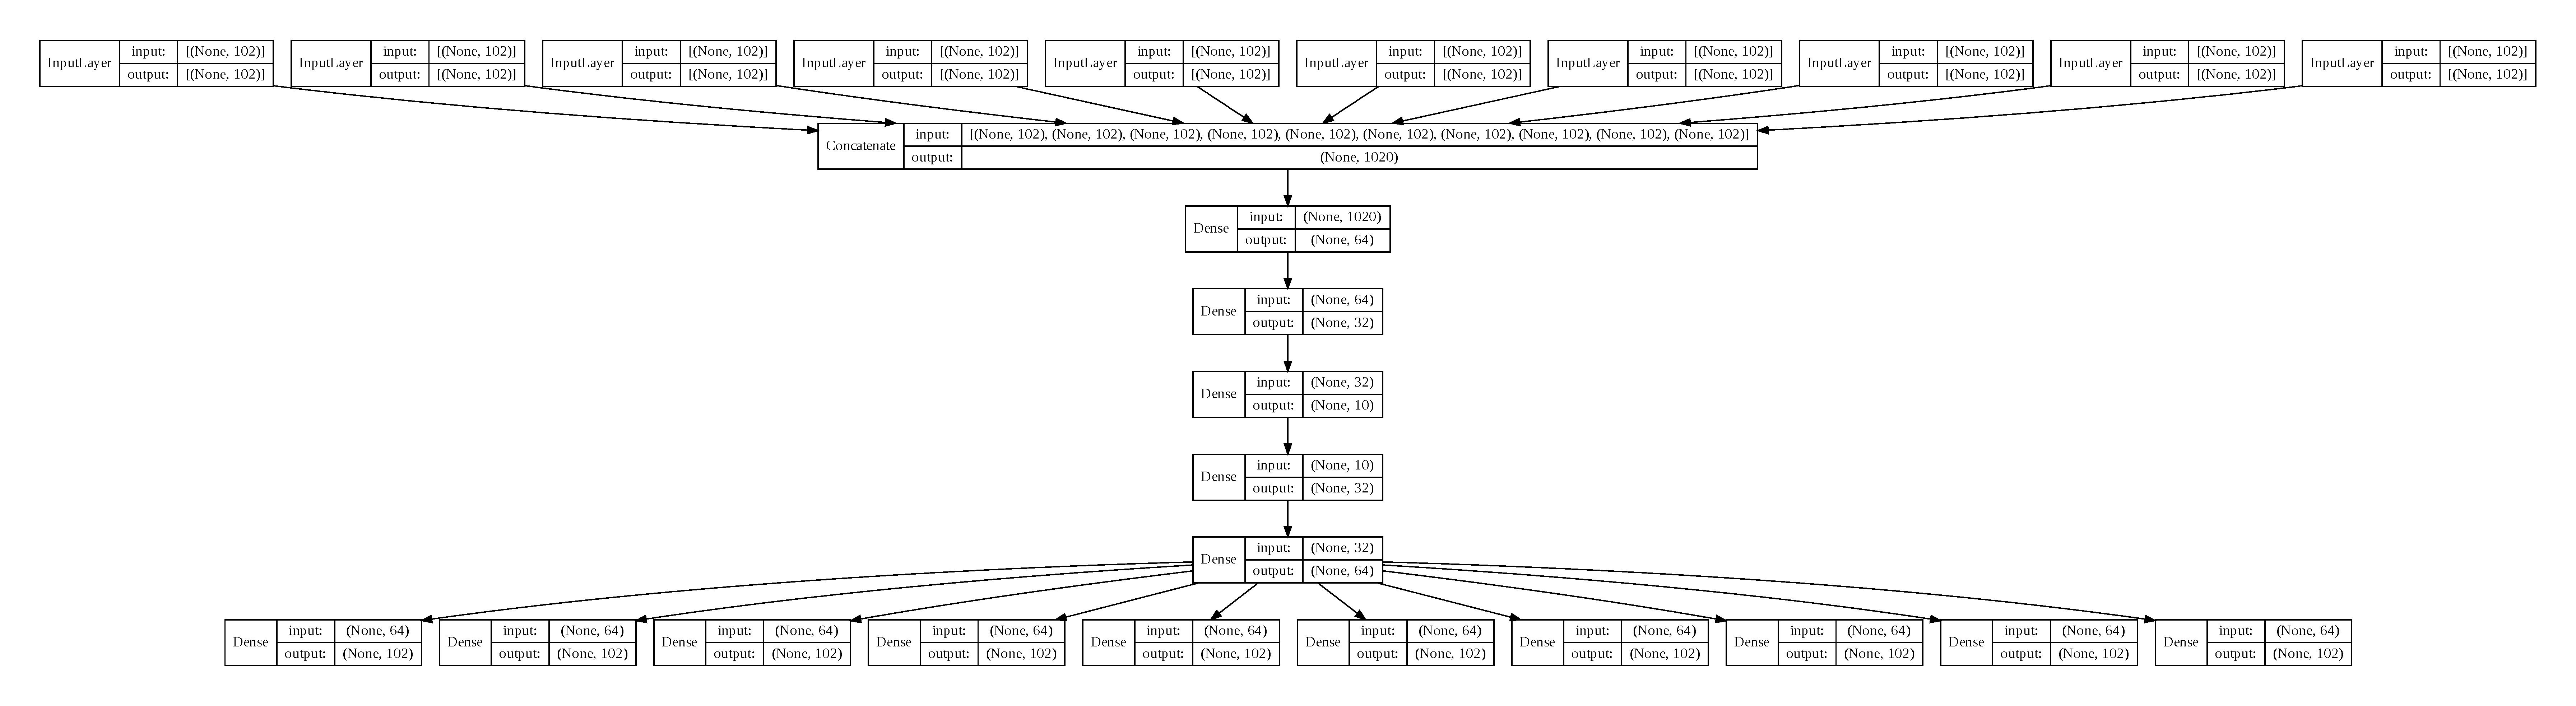
\includegraphics[width=\linewidth]{pdfs/modelTB.pdf}
\end{frame}
\end{document}
